% Chapter 8: Volatility estimators
% Statistics of Financial Markets -- Bachelor's programme, Bucharest University of Economic Studies
% GENERATED by latex/build_chapter8.py -- edit the generator, not this file.

\newcommand{\coursename}{Statistics of Financial Markets}
% Preambul comun SFM -- Statistica piețelor financiare / Statistics of Financial Markets (Beamer, 16:9)
% Același design ca MFM. Înainte de % Preambul comun SFM -- Statistica piețelor financiare / Statistics of Financial Markets (Beamer, 16:9)
% Același design ca MFM. Înainte de % Preambul comun SFM -- Statistica piețelor financiare / Statistics of Financial Markets (Beamer, 16:9)
% Același design ca MFM. Înainte de \input{../../latex/preamble} se definește
%   \newcommand{\coursename}{Statistics of Financial Markets}      (EN)
%   \newcommand{\coursename}{Statistica piețelor financiare}       (RO)  și  \def\sfmlang{ro}
% Fișierele .tex se află în EN/Courses, EN/Seminars, RO/Cursuri, RO/Seminarii (două niveluri sub rădăcină).
% Deck-urile sînt generate de latex/build_chapterN.py / build_seminarN.py (vezi latex/sfm_build.py).

\documentclass[9pt, aspectratio=169, t]{beamer}
\providecommand{\coursename}{Statistics of Financial Markets}

% Ensure content fits on slides
\setbeamersize{text margin left=8mm, text margin right=8mm}

%=============================================================================
% THEME AND STYLE CONFIGURATION
%=============================================================================
\usetheme{default}
% Using default theme for clean header/footer control

% Color Palette (matching Redispatch PDF)
\definecolor{MainBlue}{RGB}{26, 58, 110}
\definecolor{AccentBlue}{RGB}{26, 58, 110}
\definecolor{IDAred}{RGB}{205, 0, 0}
\definecolor{DarkGray}{RGB}{51, 51, 51}
\definecolor{MediumGray}{RGB}{128, 128, 128}
\definecolor{LightGray}{RGB}{248, 248, 248}
\definecolor{VeryLightGray}{RGB}{235, 235, 235}
\definecolor{KeynoteGray}{RGB}{218, 218, 218}
\definecolor{SectionGray}{RGB}{120, 120, 120}
\definecolor{FooterGray}{RGB}{100, 100, 100}
\definecolor{Crimson}{RGB}{220, 53, 69}
\definecolor{Forest}{RGB}{46, 125, 50}
\definecolor{Amber}{RGB}{181, 133, 63}
\definecolor{Orange}{RGB}{230, 126, 34}
\definecolor{Purple}{RGB}{142, 68, 173}

% Gradient background (exact Keynote 315° gradient: white to RGB 218,218,218)
\setbeamertemplate{background}{%
    \begin{tikzpicture}[remember picture, overlay]
        \shade[shading=axis, shading angle=315,
        top color=white, bottom color=KeynoteGray]
        (current page.south west) rectangle (current page.north east);
    \end{tikzpicture}%
}
% Fallback solid color for compatibility
\setbeamercolor{background canvas}{bg=}

\setbeamercolor{palette primary}{bg=MainBlue, fg=white}
\setbeamercolor{palette secondary}{bg=MainBlue!85, fg=white}
\setbeamercolor{palette tertiary}{bg=MainBlue!70, fg=white}
\setbeamercolor{structure}{fg=MainBlue}
\setbeamercolor{title}{fg=IDAred}
\setbeamercolor{frametitle}{fg=IDAred, bg=}
\setbeamercolor{block title}{bg=MainBlue, fg=white}
\setbeamercolor{block body}{bg=VeryLightGray, fg=DarkGray}
\setbeamercolor{block title alerted}{bg=Crimson, fg=white}
\setbeamercolor{block body alerted}{bg=Crimson!8, fg=DarkGray}
\setbeamercolor{block title example}{bg=Forest, fg=white}
\setbeamercolor{block body example}{bg=Forest!8, fg=DarkGray}
\setbeamercolor{item}{fg=MainBlue}

% Footer colors (override Madrid theme blue)
\setbeamercolor{author in head/foot}{fg=FooterGray, bg=}
\setbeamercolor{title in head/foot}{fg=FooterGray, bg=}
\setbeamercolor{date in head/foot}{fg=FooterGray, bg=}
\setbeamercolor{section in head/foot}{fg=FooterGray, bg=}
\setbeamercolor{subsection in head/foot}{fg=FooterGray, bg=}

% Bullet styles (apply everywhere including blocks)
\setbeamertemplate{itemize item}{\color{MainBlue}$\boxdot$}
\setbeamertemplate{itemize subitem}{\color{MainBlue}$\blacktriangleright$}
\setbeamertemplate{itemize subsubitem}{\color{MainBlue}\tiny$\bullet$}
\setbeamertemplate{itemize/enumerate body begin}{\normalsize}
\setbeamertemplate{itemize/enumerate subbody begin}{\normalsize}

% Item spacing - compact style
\setlength{\leftmargini}{10pt}       % Level 1: minimal indent
\setlength{\leftmarginii}{10pt}      % Level 2: minimal additional indent
% Compact list spacing (zero extra space before/after lists in blocks)
\makeatletter
\def\@listi{\leftmargin\leftmargini \topsep 0pt \parsep 0pt \itemsep 0pt}
\def\@listii{\leftmargin\leftmarginii \topsep 0pt \parsep 0pt \itemsep 0pt}
\makeatother

\setbeamertemplate{navigation symbols}{}

%=============================================================================
% CUSTOM HEADLINE
%=============================================================================
\setbeamertemplate{headline}{%
    \vskip10pt%
    \hbox to \paperwidth{%
        \hskip0.5cm%
        {\small\color{FooterGray}\renewcommand{\hyperlink}[2]{##2}\insertsectionhead}%
        \hfill%
        \textcolor{FooterGray}{\small\insertframenumber}%
        \hskip0.5cm%
    }%
    \vskip4pt%
    {\color{FooterGray}\hrule height 0.4pt}%
}

%=============================================================================
% CUSTOM FOOTER
%=============================================================================
\usepackage{fontawesome5}

\setbeamertemplate{footline}{%
    {\color{FooterGray}\hrule height 0.4pt}%
    \vskip4pt%
    \hbox to \paperwidth{%
        \hskip0.5cm%
        \textcolor{FooterGray}{\small\coursename}%
        \hfill%
        \raisebox{-0.1em}{%
            \begin{tikzpicture}[x=0.08em, y=0.08em, line width=0.4pt]
                \draw[FooterGray] (0,3) -- (1,4) -- (2,3.5) -- (3,5) -- (4,4) -- (5,6) -- (6,5.5) -- (7,4) -- (8,5) -- (9,7) -- (10,6) -- (11,5) -- (12,6.5) -- (13,8) -- (14,7) -- (15,6) -- (16,7.5) -- (17,9) -- (18,8) -- (19,7) -- (20,8.5) -- (21,10) -- (22,9) -- (23,8) -- (24,9.5);
            \end{tikzpicture}%
        }%
        \hskip0.5cm%
    }%
    \vskip6pt%
}

%=============================================================================
% PACKAGES
%=============================================================================
\usepackage[utf8]{inputenc}
\DeclareUnicodeCharacter{03B1}{\ensuremath{\alpha}}
\usepackage[T1]{fontenc}
\usepackage{amsmath, amssymb, amsthm}
\usepackage{mathtools}
\usepackage{bm}
\usepackage{tikz}
\usetikzlibrary{arrows.meta, positioning, shapes, calc, decorations.pathreplacing, shadings}
\usepackage{booktabs}
\usepackage{multirow}
\usepackage{array}
\usepackage{graphicx}
\usepackage{hyperref}
\usepackage{colortbl}
\usepackage{listings}
\lstset{language=Python, basicstyle=\ttfamily\scriptsize, keywordstyle=\color{MainBlue}\bfseries,
  commentstyle=\color{Forest}, stringstyle=\color{Crimson}, breaklines=true,
  frame=none, backgroundcolor=\color{VeryLightGray}, xleftmargin=2mm}
\hypersetup{colorlinks=true, linkcolor=MainBlue, urlcolor=MainBlue}
\graphicspath{{../../logos/}{../../charts/}{../../photos/}}
\usepackage{xcolor}
\hfuzz=2pt  % Suppress tiny overfull warnings (<2pt)
\vfuzz=2pt  % Suppress tiny vertical overfull warnings (<2pt)

%=============================================================================
% QUANTLET COMMANDS
%   \quantlet{<displayed name>}{<url>}       (generic, compatible with the older SFM decks)
%   \sfmquantlet{Ch_05}{SFM_ch5_garch}       -> https://github.com/danpele/SFM/tree/main/Quantlets/Ch_05/SFM_ch5_garch
%   \qlurl{<folder>} is defined per chapter by the generator (Quantlets/Ch_NN/<folder>)
%=============================================================================
\newcommand{\sfmrepo}{https://github.com/danpele/SFM}
\newcommand{\sfmqlbase}{https://github.com/danpele/SFM/tree/main/Quantlets}
\newcommand{\quantlet}[2]{%
    \hfill\href{#2}{%
        \raisebox{-0.15em}{
\includegraphics[height=0.7em]{ql_logo.png}}%
        \textcolor{MainBlue}{\tiny\ #1}%
    }%
}
\newcommand{\sfmquantlet}[2]{\quantlet{\detokenize{#2}}{\sfmqlbase/#1/#2}}

%=============================================================================
% NOTEBOOKS (Google Colab)
%   \colaburl{notebooks/EN/chapter5_seminar_notebook.ipynb} -> the Colab link of a file in the SFM repo
%   \nb: the chapter notebook (each seminar deck redefines it with \renewcommand)
%=============================================================================
\newcommand{\colaburl}[1]{https://colab.research.google.com/github/danpele/SFM/blob/main/#1}
\newcommand{\nb}{https://colab.research.google.com/github/danpele/SFM/tree/main/notebooks/EN}
\newcommand{\nbname}{notebooks/EN}

%=============================================================================
% SLIDE HELPERS (used by the generators; the same as in MFM)
%=============================================================================
% local font size for list bodies (the preamble forces \normalsize)
\newcommand{\itemsize}[1]{\setbeamertemplate{itemize/enumerate body begin}{#1}\setbeamertemplate{itemize/enumerate subbody begin}{#1}}
\newcommand{\intitle}[1]{{\hypersetup{urlcolor=white}#1}}   % white links inside coloured title bars
\newcommand{\imgcap}[1]{{\scriptsize #1}\\[0.5mm]}          % caption under a photo
\newcommand{\imgcredit}[2]{{\tiny\color{FooterGray}\href{#1}{#2}}}   % image credit: source URL, author/licence
\newcommand{\aiprompt}[1]{{\ttfamily\color{MainBlue}#1}}     % a prompt to an AI assistant

%=============================================================================
% SEMINARS: student version by default; the instructor wrapper *_solutions.tex sets \solutionstrue
%=============================================================================
\makeatletter\@ifundefined{ifsolutions}{\expandafter\newif\csname ifsolutions\endcsname}{}\makeatother
\newcommand{\solonly}[1]{\ifsolutions #1\fi}
\newcommand{\propsub}{\ifsolutions\else\framesubtitle{\ifdefined\sfmlang Rezolvarea se discută la seminar\else Solution discussed in class\fi}\fi}

%=============================================================================
% APPENDIX AND CHAPTER LINKS (latex/appendix_links.py writes the calls; it also re-declares these
% macros before \begin{document}, so the decks compile with or without this preamble block)
%=============================================================================
\providecommand{\sfmapplink}[3]{\hypertarget{#2}{}\hyperlink{#1}{\beamergotobutton{#3}}}
\providecommand{\sfmappback}[2]{\begin{tikzpicture}[remember picture,overlay]\node[anchor=south east] at ([xshift=-3mm,yshift=7mm]current page.south east){\hyperlink{#1}{\beamerreturnbutton{#2}}};\end{tikzpicture}}
\providecommand{\sfmchlink}[2]{\href{#1}{#2}}
\providecommand{\sfmchlinkt}[2]{\href{#1}{\usebeamercolor[fg]{frametitle}#2}}

%=============================================================================
% QUANTINAR COMMAND: link către un curs Quantinar (subiecte avansate)
%=============================================================================
\newcommand{\quantinar}[2]{%
    \href{#2}{%
        \raisebox{-0.15em}{
\includegraphics[height=0.8em]{qr_logo.png}}%
        \textcolor{MainBlue}{\scriptsize\ #1}%
    }%
}

%=============================================================================
% CUSTOM TITLE PAGE
%=============================================================================
\defbeamertemplate*{title page}{hybrid}[1][]
{
    \vspace{0.2cm}
    % Logos row - top header (with clickable links)
    \begin{center}
        \href{https://www.ase.ro}{
\includegraphics[height=1.0cm]{ase_logo.png}}\hspace{0.3cm}%
        \href{https://theida.net}{
\includegraphics[height=1.0cm]{ida_logo.png}}\hspace{0.3cm}%
        \href{https://blockchain-research-center.com}{
\includegraphics[height=1.0cm]{brc_logo.png}}\hspace{0.3cm}%
        \href{https://www.ai4efin.ase.ro}{
\includegraphics[height=1.0cm]{ai4efin_logo.png}}\hspace{0.3cm}%
        \href{https://ipe.ro/new}{
\includegraphics[height=1.0cm]{acad_logo.png}}\hspace{0.3cm}%
        \href{https://www.digital-finance-msca.com}{
\includegraphics[height=1.0cm]{msca_logo.png}}%
    \end{center}

    \vspace{0.6cm}

    % Main title with Q logos on sides (with clickable links)
    \begin{center}
        \begin{minipage}{0.1\textwidth}
            \centering
            \href{https://quantlet.com}{
\includegraphics[height=1.1cm]{ql_logo.png}}
        \end{minipage}%
        \begin{minipage}{0.78\textwidth}
            \centering
            {\LARGE\bfseries\usebeamercolor[fg]{title}\inserttitle}

            \vspace{0.3cm}

            {\usebeamerfont{subtitle}\usebeamercolor[fg]{title}\insertsubtitle}
        \end{minipage}%
        \begin{minipage}{0.1\textwidth}
            \centering
            \href{https://quantinar.com}{
\includegraphics[height=1.1cm]{qr_logo.png}}
        \end{minipage}
    \end{center}

    \vspace{0.6cm}

    % Authors (left aligned)
    \hspace{0.5cm}{\usebeamerfont{author}\insertauthor}

    \vspace{0.3cm}

    % Institute/Affiliations (left aligned)
    \hspace{0.5cm}\begin{minipage}[t]{0.9\textwidth}
        \raggedright\small\insertinstitute
    \end{minipage}
}

%=============================================================================
% THEOREM ENVIRONMENTS
%=============================================================================
\theoremstyle{definition}
\setbeamertemplate{theorems}[numbered]
\ifdefined\sfmlang
\newtheorem{defn}{Definiție}
\newtheorem{thm}{Teoremă}
\newtheorem{prop}{Propoziție}
\newtheorem{rmk}{Observație}
\else
\newtheorem{defn}{Definition}
\newtheorem{thm}{Theorem}
\newtheorem{prop}{Proposition}
\newtheorem{rmk}{Remark}
\fi

%=============================================================================
% CENTRED MINIPAGE (no extra vertical space)
%=============================================================================
\newenvironment{cminipage}[1]{%
    \par\noindent\hfill\begin{minipage}{#1}\ignorespaces
}{%
    \end{minipage}\hfill\null\par
}

%=============================================================================
% CUSTOM COMMANDS
%=============================================================================
\newcommand{\E}{\mathbb{E}}
\newcommand{\Var}{\text{Var}}
\newcommand{\Cov}{\text{Cov}}
\newcommand{\Corr}{\text{Corr}}
\newcommand{\R}{\mathbb{R}}
\newcommand{\N}{\mathbb{N}}
\newcommand{\Z}{\mathbb{Z}}
\newcommand{\B}{\mathbf{B}}
\newcommand{\imark}{\textcolor{MainBlue}{\textbullet}}
\newcommand{\RMSE}{\text{RMSE}}
\newcommand{\MAE}{\text{MAE}}
\newcommand{\MAPE}{\text{MAPE}}

 se definește
%   \newcommand{\coursename}{Statistics of Financial Markets}      (EN)
%   \newcommand{\coursename}{Statistica piețelor financiare}       (RO)  și  \def\sfmlang{ro}
% Fișierele .tex se află în EN/Courses, EN/Seminars, RO/Cursuri, RO/Seminarii (două niveluri sub rădăcină).
% Deck-urile sînt generate de latex/build_chapterN.py / build_seminarN.py (vezi latex/sfm_build.py).

\documentclass[9pt, aspectratio=169, t]{beamer}
\providecommand{\coursename}{Statistics of Financial Markets}

% Ensure content fits on slides
\setbeamersize{text margin left=8mm, text margin right=8mm}

%=============================================================================
% THEME AND STYLE CONFIGURATION
%=============================================================================
\usetheme{default}
% Using default theme for clean header/footer control

% Color Palette (matching Redispatch PDF)
\definecolor{MainBlue}{RGB}{26, 58, 110}
\definecolor{AccentBlue}{RGB}{26, 58, 110}
\definecolor{IDAred}{RGB}{205, 0, 0}
\definecolor{DarkGray}{RGB}{51, 51, 51}
\definecolor{MediumGray}{RGB}{128, 128, 128}
\definecolor{LightGray}{RGB}{248, 248, 248}
\definecolor{VeryLightGray}{RGB}{235, 235, 235}
\definecolor{KeynoteGray}{RGB}{218, 218, 218}
\definecolor{SectionGray}{RGB}{120, 120, 120}
\definecolor{FooterGray}{RGB}{100, 100, 100}
\definecolor{Crimson}{RGB}{220, 53, 69}
\definecolor{Forest}{RGB}{46, 125, 50}
\definecolor{Amber}{RGB}{181, 133, 63}
\definecolor{Orange}{RGB}{230, 126, 34}
\definecolor{Purple}{RGB}{142, 68, 173}

% Gradient background (exact Keynote 315° gradient: white to RGB 218,218,218)
\setbeamertemplate{background}{%
    \begin{tikzpicture}[remember picture, overlay]
        \shade[shading=axis, shading angle=315,
        top color=white, bottom color=KeynoteGray]
        (current page.south west) rectangle (current page.north east);
    \end{tikzpicture}%
}
% Fallback solid color for compatibility
\setbeamercolor{background canvas}{bg=}

\setbeamercolor{palette primary}{bg=MainBlue, fg=white}
\setbeamercolor{palette secondary}{bg=MainBlue!85, fg=white}
\setbeamercolor{palette tertiary}{bg=MainBlue!70, fg=white}
\setbeamercolor{structure}{fg=MainBlue}
\setbeamercolor{title}{fg=IDAred}
\setbeamercolor{frametitle}{fg=IDAred, bg=}
\setbeamercolor{block title}{bg=MainBlue, fg=white}
\setbeamercolor{block body}{bg=VeryLightGray, fg=DarkGray}
\setbeamercolor{block title alerted}{bg=Crimson, fg=white}
\setbeamercolor{block body alerted}{bg=Crimson!8, fg=DarkGray}
\setbeamercolor{block title example}{bg=Forest, fg=white}
\setbeamercolor{block body example}{bg=Forest!8, fg=DarkGray}
\setbeamercolor{item}{fg=MainBlue}

% Footer colors (override Madrid theme blue)
\setbeamercolor{author in head/foot}{fg=FooterGray, bg=}
\setbeamercolor{title in head/foot}{fg=FooterGray, bg=}
\setbeamercolor{date in head/foot}{fg=FooterGray, bg=}
\setbeamercolor{section in head/foot}{fg=FooterGray, bg=}
\setbeamercolor{subsection in head/foot}{fg=FooterGray, bg=}

% Bullet styles (apply everywhere including blocks)
\setbeamertemplate{itemize item}{\color{MainBlue}$\boxdot$}
\setbeamertemplate{itemize subitem}{\color{MainBlue}$\blacktriangleright$}
\setbeamertemplate{itemize subsubitem}{\color{MainBlue}\tiny$\bullet$}
\setbeamertemplate{itemize/enumerate body begin}{\normalsize}
\setbeamertemplate{itemize/enumerate subbody begin}{\normalsize}

% Item spacing - compact style
\setlength{\leftmargini}{10pt}       % Level 1: minimal indent
\setlength{\leftmarginii}{10pt}      % Level 2: minimal additional indent
% Compact list spacing (zero extra space before/after lists in blocks)
\makeatletter
\def\@listi{\leftmargin\leftmargini \topsep 0pt \parsep 0pt \itemsep 0pt}
\def\@listii{\leftmargin\leftmarginii \topsep 0pt \parsep 0pt \itemsep 0pt}
\makeatother

\setbeamertemplate{navigation symbols}{}

%=============================================================================
% CUSTOM HEADLINE
%=============================================================================
\setbeamertemplate{headline}{%
    \vskip10pt%
    \hbox to \paperwidth{%
        \hskip0.5cm%
        {\small\color{FooterGray}\renewcommand{\hyperlink}[2]{##2}\insertsectionhead}%
        \hfill%
        \textcolor{FooterGray}{\small\insertframenumber}%
        \hskip0.5cm%
    }%
    \vskip4pt%
    {\color{FooterGray}\hrule height 0.4pt}%
}

%=============================================================================
% CUSTOM FOOTER
%=============================================================================
\usepackage{fontawesome5}

\setbeamertemplate{footline}{%
    {\color{FooterGray}\hrule height 0.4pt}%
    \vskip4pt%
    \hbox to \paperwidth{%
        \hskip0.5cm%
        \textcolor{FooterGray}{\small\coursename}%
        \hfill%
        \raisebox{-0.1em}{%
            \begin{tikzpicture}[x=0.08em, y=0.08em, line width=0.4pt]
                \draw[FooterGray] (0,3) -- (1,4) -- (2,3.5) -- (3,5) -- (4,4) -- (5,6) -- (6,5.5) -- (7,4) -- (8,5) -- (9,7) -- (10,6) -- (11,5) -- (12,6.5) -- (13,8) -- (14,7) -- (15,6) -- (16,7.5) -- (17,9) -- (18,8) -- (19,7) -- (20,8.5) -- (21,10) -- (22,9) -- (23,8) -- (24,9.5);
            \end{tikzpicture}%
        }%
        \hskip0.5cm%
    }%
    \vskip6pt%
}

%=============================================================================
% PACKAGES
%=============================================================================
\usepackage[utf8]{inputenc}
\DeclareUnicodeCharacter{03B1}{\ensuremath{\alpha}}
\usepackage[T1]{fontenc}
\usepackage{amsmath, amssymb, amsthm}
\usepackage{mathtools}
\usepackage{bm}
\usepackage{tikz}
\usetikzlibrary{arrows.meta, positioning, shapes, calc, decorations.pathreplacing, shadings}
\usepackage{booktabs}
\usepackage{multirow}
\usepackage{array}
\usepackage{graphicx}
\usepackage{hyperref}
\usepackage{colortbl}
\usepackage{listings}
\lstset{language=Python, basicstyle=\ttfamily\scriptsize, keywordstyle=\color{MainBlue}\bfseries,
  commentstyle=\color{Forest}, stringstyle=\color{Crimson}, breaklines=true,
  frame=none, backgroundcolor=\color{VeryLightGray}, xleftmargin=2mm}
\hypersetup{colorlinks=true, linkcolor=MainBlue, urlcolor=MainBlue}
\graphicspath{{../../logos/}{../../charts/}{../../photos/}}
\usepackage{xcolor}
\hfuzz=2pt  % Suppress tiny overfull warnings (<2pt)
\vfuzz=2pt  % Suppress tiny vertical overfull warnings (<2pt)

%=============================================================================
% QUANTLET COMMANDS
%   \quantlet{<displayed name>}{<url>}       (generic, compatible with the older SFM decks)
%   \sfmquantlet{Ch_05}{SFM_ch5_garch}       -> https://github.com/danpele/SFM/tree/main/Quantlets/Ch_05/SFM_ch5_garch
%   \qlurl{<folder>} is defined per chapter by the generator (Quantlets/Ch_NN/<folder>)
%=============================================================================
\newcommand{\sfmrepo}{https://github.com/danpele/SFM}
\newcommand{\sfmqlbase}{https://github.com/danpele/SFM/tree/main/Quantlets}
\newcommand{\quantlet}[2]{%
    \hfill\href{#2}{%
        \raisebox{-0.15em}{
\includegraphics[height=0.7em]{ql_logo.png}}%
        \textcolor{MainBlue}{\tiny\ #1}%
    }%
}
\newcommand{\sfmquantlet}[2]{\quantlet{\detokenize{#2}}{\sfmqlbase/#1/#2}}

%=============================================================================
% NOTEBOOKS (Google Colab)
%   \colaburl{notebooks/EN/chapter5_seminar_notebook.ipynb} -> the Colab link of a file in the SFM repo
%   \nb: the chapter notebook (each seminar deck redefines it with \renewcommand)
%=============================================================================
\newcommand{\colaburl}[1]{https://colab.research.google.com/github/danpele/SFM/blob/main/#1}
\newcommand{\nb}{https://colab.research.google.com/github/danpele/SFM/tree/main/notebooks/EN}
\newcommand{\nbname}{notebooks/EN}

%=============================================================================
% SLIDE HELPERS (used by the generators; the same as in MFM)
%=============================================================================
% local font size for list bodies (the preamble forces \normalsize)
\newcommand{\itemsize}[1]{\setbeamertemplate{itemize/enumerate body begin}{#1}\setbeamertemplate{itemize/enumerate subbody begin}{#1}}
\newcommand{\intitle}[1]{{\hypersetup{urlcolor=white}#1}}   % white links inside coloured title bars
\newcommand{\imgcap}[1]{{\scriptsize #1}\\[0.5mm]}          % caption under a photo
\newcommand{\imgcredit}[2]{{\tiny\color{FooterGray}\href{#1}{#2}}}   % image credit: source URL, author/licence
\newcommand{\aiprompt}[1]{{\ttfamily\color{MainBlue}#1}}     % a prompt to an AI assistant

%=============================================================================
% SEMINARS: student version by default; the instructor wrapper *_solutions.tex sets \solutionstrue
%=============================================================================
\makeatletter\@ifundefined{ifsolutions}{\expandafter\newif\csname ifsolutions\endcsname}{}\makeatother
\newcommand{\solonly}[1]{\ifsolutions #1\fi}
\newcommand{\propsub}{\ifsolutions\else\framesubtitle{\ifdefined\sfmlang Rezolvarea se discută la seminar\else Solution discussed in class\fi}\fi}

%=============================================================================
% APPENDIX AND CHAPTER LINKS (latex/appendix_links.py writes the calls; it also re-declares these
% macros before \begin{document}, so the decks compile with or without this preamble block)
%=============================================================================
\providecommand{\sfmapplink}[3]{\hypertarget{#2}{}\hyperlink{#1}{\beamergotobutton{#3}}}
\providecommand{\sfmappback}[2]{\begin{tikzpicture}[remember picture,overlay]\node[anchor=south east] at ([xshift=-3mm,yshift=7mm]current page.south east){\hyperlink{#1}{\beamerreturnbutton{#2}}};\end{tikzpicture}}
\providecommand{\sfmchlink}[2]{\href{#1}{#2}}
\providecommand{\sfmchlinkt}[2]{\href{#1}{\usebeamercolor[fg]{frametitle}#2}}

%=============================================================================
% QUANTINAR COMMAND: link către un curs Quantinar (subiecte avansate)
%=============================================================================
\newcommand{\quantinar}[2]{%
    \href{#2}{%
        \raisebox{-0.15em}{
\includegraphics[height=0.8em]{qr_logo.png}}%
        \textcolor{MainBlue}{\scriptsize\ #1}%
    }%
}

%=============================================================================
% CUSTOM TITLE PAGE
%=============================================================================
\defbeamertemplate*{title page}{hybrid}[1][]
{
    \vspace{0.2cm}
    % Logos row - top header (with clickable links)
    \begin{center}
        \href{https://www.ase.ro}{
\includegraphics[height=1.0cm]{ase_logo.png}}\hspace{0.3cm}%
        \href{https://theida.net}{
\includegraphics[height=1.0cm]{ida_logo.png}}\hspace{0.3cm}%
        \href{https://blockchain-research-center.com}{
\includegraphics[height=1.0cm]{brc_logo.png}}\hspace{0.3cm}%
        \href{https://www.ai4efin.ase.ro}{
\includegraphics[height=1.0cm]{ai4efin_logo.png}}\hspace{0.3cm}%
        \href{https://ipe.ro/new}{
\includegraphics[height=1.0cm]{acad_logo.png}}\hspace{0.3cm}%
        \href{https://www.digital-finance-msca.com}{
\includegraphics[height=1.0cm]{msca_logo.png}}%
    \end{center}

    \vspace{0.6cm}

    % Main title with Q logos on sides (with clickable links)
    \begin{center}
        \begin{minipage}{0.1\textwidth}
            \centering
            \href{https://quantlet.com}{
\includegraphics[height=1.1cm]{ql_logo.png}}
        \end{minipage}%
        \begin{minipage}{0.78\textwidth}
            \centering
            {\LARGE\bfseries\usebeamercolor[fg]{title}\inserttitle}

            \vspace{0.3cm}

            {\usebeamerfont{subtitle}\usebeamercolor[fg]{title}\insertsubtitle}
        \end{minipage}%
        \begin{minipage}{0.1\textwidth}
            \centering
            \href{https://quantinar.com}{
\includegraphics[height=1.1cm]{qr_logo.png}}
        \end{minipage}
    \end{center}

    \vspace{0.6cm}

    % Authors (left aligned)
    \hspace{0.5cm}{\usebeamerfont{author}\insertauthor}

    \vspace{0.3cm}

    % Institute/Affiliations (left aligned)
    \hspace{0.5cm}\begin{minipage}[t]{0.9\textwidth}
        \raggedright\small\insertinstitute
    \end{minipage}
}

%=============================================================================
% THEOREM ENVIRONMENTS
%=============================================================================
\theoremstyle{definition}
\setbeamertemplate{theorems}[numbered]
\ifdefined\sfmlang
\newtheorem{defn}{Definiție}
\newtheorem{thm}{Teoremă}
\newtheorem{prop}{Propoziție}
\newtheorem{rmk}{Observație}
\else
\newtheorem{defn}{Definition}
\newtheorem{thm}{Theorem}
\newtheorem{prop}{Proposition}
\newtheorem{rmk}{Remark}
\fi

%=============================================================================
% CENTRED MINIPAGE (no extra vertical space)
%=============================================================================
\newenvironment{cminipage}[1]{%
    \par\noindent\hfill\begin{minipage}{#1}\ignorespaces
}{%
    \end{minipage}\hfill\null\par
}

%=============================================================================
% CUSTOM COMMANDS
%=============================================================================
\newcommand{\E}{\mathbb{E}}
\newcommand{\Var}{\text{Var}}
\newcommand{\Cov}{\text{Cov}}
\newcommand{\Corr}{\text{Corr}}
\newcommand{\R}{\mathbb{R}}
\newcommand{\N}{\mathbb{N}}
\newcommand{\Z}{\mathbb{Z}}
\newcommand{\B}{\mathbf{B}}
\newcommand{\imark}{\textcolor{MainBlue}{\textbullet}}
\newcommand{\RMSE}{\text{RMSE}}
\newcommand{\MAE}{\text{MAE}}
\newcommand{\MAPE}{\text{MAPE}}

 se definește
%   \newcommand{\coursename}{Statistics of Financial Markets}      (EN)
%   \newcommand{\coursename}{Statistica piețelor financiare}       (RO)  și  \def\sfmlang{ro}
% Fișierele .tex se află în EN/Courses, EN/Seminars, RO/Cursuri, RO/Seminarii (două niveluri sub rădăcină).
% Deck-urile sînt generate de latex/build_chapterN.py / build_seminarN.py (vezi latex/sfm_build.py).

\documentclass[9pt, aspectratio=169, t]{beamer}
\providecommand{\coursename}{Statistics of Financial Markets}

% Ensure content fits on slides
\setbeamersize{text margin left=8mm, text margin right=8mm}

%=============================================================================
% THEME AND STYLE CONFIGURATION
%=============================================================================
\usetheme{default}
% Using default theme for clean header/footer control

% Color Palette (matching Redispatch PDF)
\definecolor{MainBlue}{RGB}{26, 58, 110}
\definecolor{AccentBlue}{RGB}{26, 58, 110}
\definecolor{IDAred}{RGB}{205, 0, 0}
\definecolor{DarkGray}{RGB}{51, 51, 51}
\definecolor{MediumGray}{RGB}{128, 128, 128}
\definecolor{LightGray}{RGB}{248, 248, 248}
\definecolor{VeryLightGray}{RGB}{235, 235, 235}
\definecolor{KeynoteGray}{RGB}{218, 218, 218}
\definecolor{SectionGray}{RGB}{120, 120, 120}
\definecolor{FooterGray}{RGB}{100, 100, 100}
\definecolor{Crimson}{RGB}{220, 53, 69}
\definecolor{Forest}{RGB}{46, 125, 50}
\definecolor{Amber}{RGB}{181, 133, 63}
\definecolor{Orange}{RGB}{230, 126, 34}
\definecolor{Purple}{RGB}{142, 68, 173}

% Gradient background (exact Keynote 315° gradient: white to RGB 218,218,218)
\setbeamertemplate{background}{%
    \begin{tikzpicture}[remember picture, overlay]
        \shade[shading=axis, shading angle=315,
        top color=white, bottom color=KeynoteGray]
        (current page.south west) rectangle (current page.north east);
    \end{tikzpicture}%
}
% Fallback solid color for compatibility
\setbeamercolor{background canvas}{bg=}

\setbeamercolor{palette primary}{bg=MainBlue, fg=white}
\setbeamercolor{palette secondary}{bg=MainBlue!85, fg=white}
\setbeamercolor{palette tertiary}{bg=MainBlue!70, fg=white}
\setbeamercolor{structure}{fg=MainBlue}
\setbeamercolor{title}{fg=IDAred}
\setbeamercolor{frametitle}{fg=IDAred, bg=}
\setbeamercolor{block title}{bg=MainBlue, fg=white}
\setbeamercolor{block body}{bg=VeryLightGray, fg=DarkGray}
\setbeamercolor{block title alerted}{bg=Crimson, fg=white}
\setbeamercolor{block body alerted}{bg=Crimson!8, fg=DarkGray}
\setbeamercolor{block title example}{bg=Forest, fg=white}
\setbeamercolor{block body example}{bg=Forest!8, fg=DarkGray}
\setbeamercolor{item}{fg=MainBlue}

% Footer colors (override Madrid theme blue)
\setbeamercolor{author in head/foot}{fg=FooterGray, bg=}
\setbeamercolor{title in head/foot}{fg=FooterGray, bg=}
\setbeamercolor{date in head/foot}{fg=FooterGray, bg=}
\setbeamercolor{section in head/foot}{fg=FooterGray, bg=}
\setbeamercolor{subsection in head/foot}{fg=FooterGray, bg=}

% Bullet styles (apply everywhere including blocks)
\setbeamertemplate{itemize item}{\color{MainBlue}$\boxdot$}
\setbeamertemplate{itemize subitem}{\color{MainBlue}$\blacktriangleright$}
\setbeamertemplate{itemize subsubitem}{\color{MainBlue}\tiny$\bullet$}
\setbeamertemplate{itemize/enumerate body begin}{\normalsize}
\setbeamertemplate{itemize/enumerate subbody begin}{\normalsize}

% Item spacing - compact style
\setlength{\leftmargini}{10pt}       % Level 1: minimal indent
\setlength{\leftmarginii}{10pt}      % Level 2: minimal additional indent
% Compact list spacing (zero extra space before/after lists in blocks)
\makeatletter
\def\@listi{\leftmargin\leftmargini \topsep 0pt \parsep 0pt \itemsep 0pt}
\def\@listii{\leftmargin\leftmarginii \topsep 0pt \parsep 0pt \itemsep 0pt}
\makeatother

\setbeamertemplate{navigation symbols}{}

%=============================================================================
% CUSTOM HEADLINE
%=============================================================================
\setbeamertemplate{headline}{%
    \vskip10pt%
    \hbox to \paperwidth{%
        \hskip0.5cm%
        {\small\color{FooterGray}\renewcommand{\hyperlink}[2]{##2}\insertsectionhead}%
        \hfill%
        \textcolor{FooterGray}{\small\insertframenumber}%
        \hskip0.5cm%
    }%
    \vskip4pt%
    {\color{FooterGray}\hrule height 0.4pt}%
}

%=============================================================================
% CUSTOM FOOTER
%=============================================================================
\usepackage{fontawesome5}

\setbeamertemplate{footline}{%
    {\color{FooterGray}\hrule height 0.4pt}%
    \vskip4pt%
    \hbox to \paperwidth{%
        \hskip0.5cm%
        \textcolor{FooterGray}{\small\coursename}%
        \hfill%
        \raisebox{-0.1em}{%
            \begin{tikzpicture}[x=0.08em, y=0.08em, line width=0.4pt]
                \draw[FooterGray] (0,3) -- (1,4) -- (2,3.5) -- (3,5) -- (4,4) -- (5,6) -- (6,5.5) -- (7,4) -- (8,5) -- (9,7) -- (10,6) -- (11,5) -- (12,6.5) -- (13,8) -- (14,7) -- (15,6) -- (16,7.5) -- (17,9) -- (18,8) -- (19,7) -- (20,8.5) -- (21,10) -- (22,9) -- (23,8) -- (24,9.5);
            \end{tikzpicture}%
        }%
        \hskip0.5cm%
    }%
    \vskip6pt%
}

%=============================================================================
% PACKAGES
%=============================================================================
\usepackage[utf8]{inputenc}
\DeclareUnicodeCharacter{03B1}{\ensuremath{\alpha}}
\usepackage[T1]{fontenc}
\usepackage{amsmath, amssymb, amsthm}
\usepackage{mathtools}
\usepackage{bm}
\usepackage{tikz}
\usetikzlibrary{arrows.meta, positioning, shapes, calc, decorations.pathreplacing, shadings}
\usepackage{booktabs}
\usepackage{multirow}
\usepackage{array}
\usepackage{graphicx}
\usepackage{hyperref}
\usepackage{colortbl}
\usepackage{listings}
\lstset{language=Python, basicstyle=\ttfamily\scriptsize, keywordstyle=\color{MainBlue}\bfseries,
  commentstyle=\color{Forest}, stringstyle=\color{Crimson}, breaklines=true,
  frame=none, backgroundcolor=\color{VeryLightGray}, xleftmargin=2mm}
\hypersetup{colorlinks=true, linkcolor=MainBlue, urlcolor=MainBlue}
\graphicspath{{../../logos/}{../../charts/}{../../photos/}}
\usepackage{xcolor}
\hfuzz=2pt  % Suppress tiny overfull warnings (<2pt)
\vfuzz=2pt  % Suppress tiny vertical overfull warnings (<2pt)

%=============================================================================
% QUANTLET COMMANDS
%   \quantlet{<displayed name>}{<url>}       (generic, compatible with the older SFM decks)
%   \sfmquantlet{Ch_05}{SFM_ch5_garch}       -> https://github.com/danpele/SFM/tree/main/Quantlets/Ch_05/SFM_ch5_garch
%   \qlurl{<folder>} is defined per chapter by the generator (Quantlets/Ch_NN/<folder>)
%=============================================================================
\newcommand{\sfmrepo}{https://github.com/danpele/SFM}
\newcommand{\sfmqlbase}{https://github.com/danpele/SFM/tree/main/Quantlets}
\newcommand{\quantlet}[2]{%
    \hfill\href{#2}{%
        \raisebox{-0.15em}{
\includegraphics[height=0.7em]{ql_logo.png}}%
        \textcolor{MainBlue}{\tiny\ #1}%
    }%
}
\newcommand{\sfmquantlet}[2]{\quantlet{\detokenize{#2}}{\sfmqlbase/#1/#2}}

%=============================================================================
% NOTEBOOKS (Google Colab)
%   \colaburl{notebooks/EN/chapter5_seminar_notebook.ipynb} -> the Colab link of a file in the SFM repo
%   \nb: the chapter notebook (each seminar deck redefines it with \renewcommand)
%=============================================================================
\newcommand{\colaburl}[1]{https://colab.research.google.com/github/danpele/SFM/blob/main/#1}
\newcommand{\nb}{https://colab.research.google.com/github/danpele/SFM/tree/main/notebooks/EN}
\newcommand{\nbname}{notebooks/EN}

%=============================================================================
% SLIDE HELPERS (used by the generators; the same as in MFM)
%=============================================================================
% local font size for list bodies (the preamble forces \normalsize)
\newcommand{\itemsize}[1]{\setbeamertemplate{itemize/enumerate body begin}{#1}\setbeamertemplate{itemize/enumerate subbody begin}{#1}}
\newcommand{\intitle}[1]{{\hypersetup{urlcolor=white}#1}}   % white links inside coloured title bars
\newcommand{\imgcap}[1]{{\scriptsize #1}\\[0.5mm]}          % caption under a photo
\newcommand{\imgcredit}[2]{{\tiny\color{FooterGray}\href{#1}{#2}}}   % image credit: source URL, author/licence
\newcommand{\aiprompt}[1]{{\ttfamily\color{MainBlue}#1}}     % a prompt to an AI assistant

%=============================================================================
% SEMINARS: student version by default; the instructor wrapper *_solutions.tex sets \solutionstrue
%=============================================================================
\makeatletter\@ifundefined{ifsolutions}{\expandafter\newif\csname ifsolutions\endcsname}{}\makeatother
\newcommand{\solonly}[1]{\ifsolutions #1\fi}
\newcommand{\propsub}{\ifsolutions\else\framesubtitle{\ifdefined\sfmlang Rezolvarea se discută la seminar\else Solution discussed in class\fi}\fi}

%=============================================================================
% APPENDIX AND CHAPTER LINKS (latex/appendix_links.py writes the calls; it also re-declares these
% macros before \begin{document}, so the decks compile with or without this preamble block)
%=============================================================================
\providecommand{\sfmapplink}[3]{\hypertarget{#2}{}\hyperlink{#1}{\beamergotobutton{#3}}}
\providecommand{\sfmappback}[2]{\begin{tikzpicture}[remember picture,overlay]\node[anchor=south east] at ([xshift=-3mm,yshift=7mm]current page.south east){\hyperlink{#1}{\beamerreturnbutton{#2}}};\end{tikzpicture}}
\providecommand{\sfmchlink}[2]{\href{#1}{#2}}
\providecommand{\sfmchlinkt}[2]{\href{#1}{\usebeamercolor[fg]{frametitle}#2}}

%=============================================================================
% QUANTINAR COMMAND: link către un curs Quantinar (subiecte avansate)
%=============================================================================
\newcommand{\quantinar}[2]{%
    \href{#2}{%
        \raisebox{-0.15em}{
\includegraphics[height=0.8em]{qr_logo.png}}%
        \textcolor{MainBlue}{\scriptsize\ #1}%
    }%
}

%=============================================================================
% CUSTOM TITLE PAGE
%=============================================================================
\defbeamertemplate*{title page}{hybrid}[1][]
{
    \vspace{0.2cm}
    % Logos row - top header (with clickable links)
    \begin{center}
        \href{https://www.ase.ro}{
\includegraphics[height=1.0cm]{ase_logo.png}}\hspace{0.3cm}%
        \href{https://theida.net}{
\includegraphics[height=1.0cm]{ida_logo.png}}\hspace{0.3cm}%
        \href{https://blockchain-research-center.com}{
\includegraphics[height=1.0cm]{brc_logo.png}}\hspace{0.3cm}%
        \href{https://www.ai4efin.ase.ro}{
\includegraphics[height=1.0cm]{ai4efin_logo.png}}\hspace{0.3cm}%
        \href{https://ipe.ro/new}{
\includegraphics[height=1.0cm]{acad_logo.png}}\hspace{0.3cm}%
        \href{https://www.digital-finance-msca.com}{
\includegraphics[height=1.0cm]{msca_logo.png}}%
    \end{center}

    \vspace{0.6cm}

    % Main title with Q logos on sides (with clickable links)
    \begin{center}
        \begin{minipage}{0.1\textwidth}
            \centering
            \href{https://quantlet.com}{
\includegraphics[height=1.1cm]{ql_logo.png}}
        \end{minipage}%
        \begin{minipage}{0.78\textwidth}
            \centering
            {\LARGE\bfseries\usebeamercolor[fg]{title}\inserttitle}

            \vspace{0.3cm}

            {\usebeamerfont{subtitle}\usebeamercolor[fg]{title}\insertsubtitle}
        \end{minipage}%
        \begin{minipage}{0.1\textwidth}
            \centering
            \href{https://quantinar.com}{
\includegraphics[height=1.1cm]{qr_logo.png}}
        \end{minipage}
    \end{center}

    \vspace{0.6cm}

    % Authors (left aligned)
    \hspace{0.5cm}{\usebeamerfont{author}\insertauthor}

    \vspace{0.3cm}

    % Institute/Affiliations (left aligned)
    \hspace{0.5cm}\begin{minipage}[t]{0.9\textwidth}
        \raggedright\small\insertinstitute
    \end{minipage}
}

%=============================================================================
% THEOREM ENVIRONMENTS
%=============================================================================
\theoremstyle{definition}
\setbeamertemplate{theorems}[numbered]
\ifdefined\sfmlang
\newtheorem{defn}{Definiție}
\newtheorem{thm}{Teoremă}
\newtheorem{prop}{Propoziție}
\newtheorem{rmk}{Observație}
\else
\newtheorem{defn}{Definition}
\newtheorem{thm}{Theorem}
\newtheorem{prop}{Proposition}
\newtheorem{rmk}{Remark}
\fi

%=============================================================================
% CENTRED MINIPAGE (no extra vertical space)
%=============================================================================
\newenvironment{cminipage}[1]{%
    \par\noindent\hfill\begin{minipage}{#1}\ignorespaces
}{%
    \end{minipage}\hfill\null\par
}

%=============================================================================
% CUSTOM COMMANDS
%=============================================================================
\newcommand{\E}{\mathbb{E}}
\newcommand{\Var}{\text{Var}}
\newcommand{\Cov}{\text{Cov}}
\newcommand{\Corr}{\text{Corr}}
\newcommand{\R}{\mathbb{R}}
\newcommand{\N}{\mathbb{N}}
\newcommand{\Z}{\mathbb{Z}}
\newcommand{\B}{\mathbf{B}}
\newcommand{\imark}{\textcolor{MainBlue}{\textbullet}}
\newcommand{\RMSE}{\text{RMSE}}
\newcommand{\MAE}{\text{MAE}}
\newcommand{\MAPE}{\text{MAPE}}



\newcommand{\qlurl}[1]{https://github.com/danpele/SFM/tree/main/Quantlets/Ch_08/#1}

% Clickable citations (DOIs verified via Crossref)

\newcommand{\refFHH}{\href{https://doi.org/10.1007/978-3-030-13751-9}{Franke, Härdle \& Hafner (2019)}}
\newcommand{\refBHL}{\href{https://doi.org/10.1007/978-3-642-33929-5}{Borak, Härdle \& López-Cabrera (2013)}}
\newcommand{\refTsay}{\href{https://doi.org/10.1002/9780470644560}{Tsay (2010)}}
\newcommand{\refMandelbrot}{\href{https://doi.org/10.1086/294632}{Mandelbrot (1963)}}
\newcommand{\refCont}{\href{https://doi.org/10.1080/713665670}{Cont (2001)}}
\newcommand{\refEngle}{\href{https://doi.org/10.2307/1912773}{Engle (1982)}}
\newcommand{\refEngleN}{\href{https://doi.org/10.1257/0002828041464597}{Engle (2004)}}
\newcommand{\refNobel}{\href{https://www.nobelprize.org/prizes/economic-sciences/2003/summary/}{Nobel Prize (2003)}}
\newcommand{\refBollerslev}{\href{https://doi.org/10.1016/0304-4076(86)90063-1}{Bollerslev (1986)}}
\newcommand{\refRM}{\href{https://www.msci.com/documents/10199/5915b101-4206-4ba0-aee2-3449d5c7e95a}{J.P. Morgan/Reuters (1996)}}
\newcommand{\refParkinson}{\href{https://doi.org/10.1086/296071}{Parkinson (1980)}}
\newcommand{\refGK}{\href{https://doi.org/10.1086/296072}{Garman \& Klass (1980)}}
\newcommand{\refRS}{\href{https://doi.org/10.1214/aoap/1177005835}{Rogers \& Satchell (1991)}}
\newcommand{\refYZ}{\href{https://doi.org/10.1086/209650}{Yang \& Zhang (2000)}}
\newcommand{\refMolnar}{\href{https://doi.org/10.1016/j.irfa.2011.06.012}{Molnár (2012)}}
\newcommand{\refABD}{\href{https://doi.org/10.1111/1540-6261.00454}{Alizadeh, Brandt \& Diebold (2002)}}
\newcommand{\refABDL}{\href{https://doi.org/10.1111/1468-0262.00418}{Andersen, Bollerslev, Diebold \& Labys (2003)}}
\newcommand{\refABDE}{\href{https://doi.org/10.1016/S0304-405X(01)00055-1}{Andersen, Bollerslev, Diebold \& Ebens (2001)}}
\newcommand{\refBNS}{\href{https://doi.org/10.1111/1467-9868.00336}{Barndorff-Nielsen \& Shephard (2002)}}
\newcommand{\refAB}{\href{https://doi.org/10.2307/2527343}{Andersen \& Bollerslev (1998)}}
\newcommand{\refLPS}{\href{https://doi.org/10.1016/j.jeconom.2015.02.008}{Liu, Patton \& Sheppard (2015)}}
\newcommand{\refCorsi}{\href{https://doi.org/10.1093/jjfinec/nbp001}{Corsi (2009)}}
\newcommand{\refML}{\href{https://doi.org/10.1111/j.1467-9892.1983.tb00373.x}{McLeod \& Li (1983)}}
\newcommand{\refLjung}{\href{https://doi.org/10.1093/biomet/65.2.297}{Ljung \& Box (1978)}}
\newcommand{\refDGE}{\href{https://doi.org/10.1016/0927-5398(93)90006-D}{Ding, Granger \& Engle (1993)}}
\newcommand{\refSchwert}{\href{https://doi.org/10.1111/j.1540-6261.1989.tb02647.x}{Schwert (1989)}}
\newcommand{\refChristie}{\href{https://doi.org/10.1016/0304-405X(82)90018-6}{Christie (1982)}}
\newcommand{\refFSS}{\href{https://doi.org/10.1016/0304-405X(87)90026-2}{French, Schwert \& Stambaugh (1987)}}
\newcommand{\refBW}{\href{https://doi.org/10.1093/rfs/13.1.1}{Bekaert \& Wu (2000)}}
\newcommand{\refWhaley}{\href{https://doi.org/10.3905/jod.1993.407868}{Whaley (1993)}}
\newcommand{\refWhaleyB}{\href{https://doi.org/10.3905/JPM.2009.35.3.098}{Whaley (2009)}}
\newcommand{\refCboe}{\href{https://www.cboe.com/tradable_products/vix/}{Cboe (2026)}}
\newcommand{\refCW}{\href{https://doi.org/10.1093/rfs/hhn038}{Carr \& Wu (2009)}}
\newcommand{\refBTZ}{\href{https://doi.org/10.1093/rfs/hhp008}{Bollerslev, Tauchen \& Zhou (2009)}}
\newcommand{\refPatton}{\href{https://doi.org/10.1016/j.jeconom.2010.03.034}{Patton (2011)}}
\newcommand{\refHL}{\href{https://doi.org/10.1002/jae.800}{Hansen \& Lunde (2005)}}
\newcommand{\refPG}{\href{https://doi.org/10.1257/002205103765762743}{Poon \& Granger (2003)}}
\newcommand{\refDM}{\href{https://doi.org/10.1080/07350015.1995.10524599}{Diebold \& Mariano (1995)}}
\newcommand{\refMZ}{\href{https://www.nber.org/books-and-chapters/economic-forecasts-and-expectations-analysis-forecasting-behavior-and-performance/evaluation-economic-forecasts}{Mincer \& Zarnowitz (1969)}}
\newcommand{\refWang}{\href{https://doi.org/10.1038/s41586-023-06221-2}{Wang et al.\ (2023)}}
\newcommand{\refPeleA}{\href{https://doi.org/10.3390/e19050226}{Pele, Lazar \& Dufour (2017)}}
\newcommand{\refPeleB}{\href{https://doi.org/10.3390/e21020102}{Pele \& Mazurencu-Marinescu-Pele (2019)}}

\title[Statistics of Financial Markets]{Statistics of Financial Markets}
\subtitle{Chapter 8: Volatility estimators}
\author[D.T. Pele]{Daniel Traian PELE}
\institute{Bucharest University of Economic Studies\\
IDA Institute Digital Assets\\
Blockchain Research Center\\
AI4EFin Artificial Intelligence for Energy Finance\\
Romanian Academy, Institute for Economic Forecasting\\
MSCA Digital Finance}
\date{}

%=============================================================================
\providecommand{\sfmapplink}[3]{\hypertarget{#2}{}\hyperlink{#1}{\beamergotobutton{#3}}}  % APPLINKS-MACROS
\providecommand{\sfmappback}[2]{\begin{tikzpicture}[remember picture,overlay]\node[anchor=south east] at ([xshift=-3mm,yshift=7mm]current page.south east){\hyperlink{#1}{\beamerreturnbutton{#2}}};\end{tikzpicture}}  % APPLINKS-MACROS
\providecommand{\sfmchlink}[2]{\href{#1}{#2}}  % APPLINKS-MACROS
\providecommand{\sfmchlinkt}[2]{\href{#1}{\usebeamercolor[fg]{frametitle}#2}}  % APPLINKS-MACROS
\begin{document}
%=============================================================================

{
\setbeamertemplate{headline}{}
\setbeamertemplate{footline}{}
\begin{frame}[noframenumbering]
    \titlepage
\end{frame}
}
% BEGIN-ACRONYMS (generat de latex/acronyms.py; nu editati manual)
\begin{frame}{Acronyms used in this material}
\setbeamertemplate{itemize/enumerate body begin}{\tiny}
\begin{columns}[T]
\begin{column}{0.49\textwidth}
\begin{itemize}\setlength{\itemsep}{0pt}
    \item \textbf{ACF}: Autocorrelation Function
    \item \textbf{AI}: Artificial Intelligence
    \item \textbf{AR}: AutoRegressive (model); in event studies: Abnormal Return
    \item \textbf{ARCH}: AutoRegressive Conditional Heteroskedasticity
    \item \textbf{ARCH-LM}: ARCH Lagrange Multiplier (test)
    \item \textbf{BET}: Bucharest Exchange Trading (index)
    \item \textbf{BVB}: Bursa de Valori București (the Bucharest Stock Exchange)
    \item \textbf{CBOE}: Chicago Board Options Exchange
    \item \textbf{DM}: Diebold–Mariano (test)
    \item \textbf{EODHD}: EOD Historical Data (market-data provider)
    \item \textbf{ES}: Expected Shortfall
    \item \textbf{EWMA}: Exponentially Weighted Moving Average
    \item \textbf{GARCH}: Generalised AutoRegressive Conditional Heteroskedasticity
\end{itemize}
\end{column}
\begin{column}{0.49\textwidth}
\begin{itemize}\setlength{\itemsep}{0pt}
    \item \textbf{GK}: Garman–Klass (volatility estimator)
    \item \textbf{HAR}: Heterogeneous AutoRegressive (model)
    \item \textbf{IGARCH}: Integrated GARCH
    \item \textbf{LM}: Lagrange Multiplier
    \item \textbf{MSE}: Mean Squared Error
    \item \textbf{MZ}: Mincer–Zarnowitz (regression)
    \item \textbf{OHLC}: Open, High, Low, Close
    \item \textbf{QLIKE}: Quasi-LIKElihood (loss function)
    \item \textbf{RV}: Realised Variance
    \item \textbf{SE}: Standard Error
    \item \textbf{SFE}: Statistics of Financial Markets, Exercises (Quantlet collection of the textbook)
    \item \textbf{VIX}: CBOE Volatility IndeX
    \item \textbf{YZ}: Yang–Zhang (volatility estimator)
\end{itemize}
\end{column}
\end{columns}
\end{frame}
% END-ACRONYMS

\begin{frame}{Today's Question and Route}
\itemsize{\small}
\begin{itemize}
    \item \textbf{Question}: how large is the risk of an asset today, if we can never observe it directly?
    \begin{itemize}
        \item \sfmchlink{https://danpele.github.io/SFM/EN/Courses/chapter7_efficient_markets_random_walk_vr.pdf}{Chapter 7}: returns are almost unpredictable, but their size is not; here we measure that size
        \item \sfmchlink{https://danpele.github.io/SFM/EN/Courses/chapter9_arch_garch_models.pdf}{Chapter 9} turns the measurements into a model (ARCH and GARCH)
    \end{itemize}
    \item \textbf{Route} of the chapter
    \begin{itemize}
        \item what volatility is and why it is latent; historical volatility and the choice of the window
        \item EWMA (RiskMetrics); range-based estimators from open, high, low and close prices
        \item realised volatility; volatility clustering and its tests
        \item long-run behaviour, the VIX, the leverage effect; how to compare volatility forecasts
    \end{itemize}
\end{itemize}
\end{frame}

\begin{frame}{Learning Outcomes}
\itemsize{\small}
\begin{itemize}
    \item Define volatility, annualise it with the actual trading frequency and explain why it is a latent quantity
    \item Compute historical and EWMA volatility and choose a window or a decay factor
    \item Compute the Parkinson, Garman--Klass, Rogers--Satchell and Yang--Zhang estimators and state their assumptions
    \item Detect volatility clustering with the ACF of squared returns, the Ljung--Box test and the ARCH-LM test
    \item Compare implied and realised volatility, and evaluate volatility forecasts with MSE and QLIKE
\end{itemize}
\end{frame}

\begin{frame}{Reading and Tools}
\itemsize{\small}
\begin{itemize}
    \item Textbook: \refFHH, Ch.~13 (introduction: volatility and conditional heteroskedasticity)
    \begin{itemize}
        \item exercises with solutions: \refBHL, Ch.~13
    \end{itemize}
    \item Volatility and its stylised facts: \refTsay, Ch.~3.1; a review of volatility forecasting: \refPG
    \item Python Quantlets of this chapter: \href{https://github.com/danpele/SFM/tree/main/Quantlets/Ch_08}{Quantlets/Ch\_08}
    \begin{itemize}
        \item ported from the SFE Quantlets SFEkurgarch (kurtosis of a GARCH process) and SFEvolnonparest (nonparametric volatility)
    \end{itemize}
    \item Lecture notebook: \href{\colaburl{notebooks/EN/chapter8_lecture_notebook.ipynb}}{open in Google Colab}
    \item Video course: \quantinar{Applied Time Series Analysis with Python}{https://quantinar.com/course/137/applied-time-series-analysis-with-python}
\end{itemize}
\end{frame}


%=============================================================================
\section{What Is Volatility?}
%=============================================================================

\begin{frame}{Volatility Comes in Bursts}
\itemsize{\small}
\begin{columns}[T]
\begin{column}{0.52\textwidth}
\begin{itemize}
    \item ``Large changes tend to be followed by large changes, of either sign, and small changes tend to be followed by small changes'' \refMandelbrot
    \begin{itemize}
        \item after the crash of 19 October 1987, markets stayed turbulent for weeks
    \end{itemize}
    \item Volatility enters almost every number in finance
    \begin{itemize}
        \item risk measures: VaR and ES (Chapter 10), the Sharpe ratio (\sfmchlink{https://danpele.github.io/SFM/EN/Courses/chapter1_data_returns_indicators.pdf}{Chapter 1})
        \item option prices, margins of exchanges, the size of positions
    \end{itemize}
    \item This chapter: how to \textbf{measure} it from prices, and how to tell whether it clusters
\end{itemize}
\end{column}
\begin{column}{0.44\textwidth}
\centering
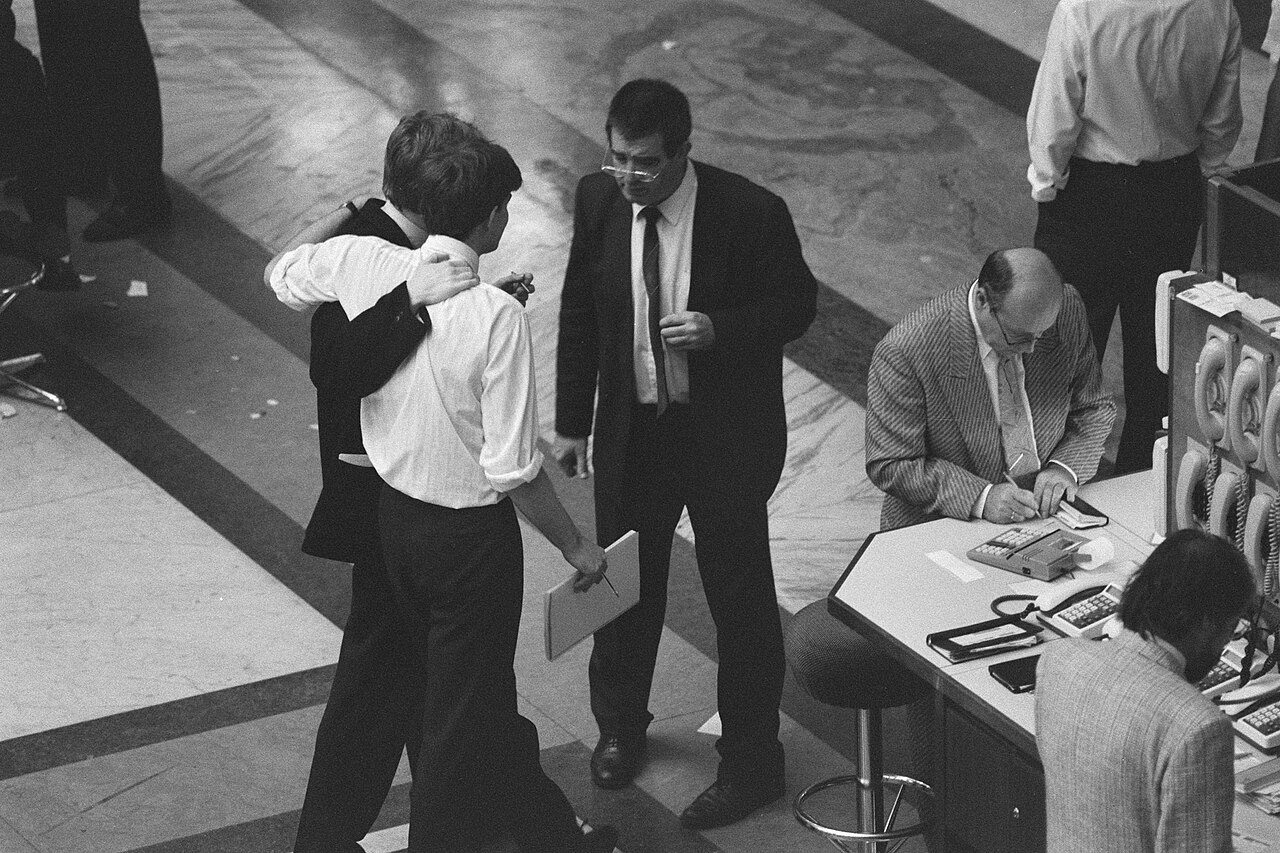
\includegraphics[height=0.36\textheight]{ch8_amsterdam_1987.jpg}\\[1mm]
\imgcap{Amsterdam Stock Exchange, 21 October 1987, two days after the crash}
\imgcredit{https://commons.wikimedia.org/wiki/File:Effectenbeurs_Amsterdam_na_koersval,_Bestanddeelnr_934-1094.jpg}{Photo: Bart Molendijk / Anefo (1987); CC0; Wikimedia Commons}
\end{column}
\end{columns}
\end{frame}

\begin{frame}{Volatility: Definition and Units}
\itemsize{\small}
\begin{itemize}
    \item Daily log return in \%: $r_t = 100\,(\ln P_t - \ln P_{t-1})$ (\sfmchlink{https://danpele.github.io/SFM/EN/Courses/chapter1_data_returns_indicators.pdf}{Chapter 1})
    \begin{itemize}
        \item \textbf{volatility} = the standard deviation of returns, $\sigma = \sqrt{\mathrm{Var}(r_t)}$
        \item it has the units of the return (\% per day); the variance $\sigma^2$ has units of \%$^2$
    \end{itemize}
    \item \textbf{Annualisation}: with $a$ observations per year and uncorrelated returns, $\sigma_{\text{year}} = \sigma_{\text{day}}\sqrt{a}$
    \begin{itemize}
        \item $a$ = the actual frequency: about 252 for the S\&P 500, 250 for the BET, 365 for Bitcoin (trades every day)
        \item the rule $\sqrt{a}$ is the square-root-of-time rule of \sfmchlink{https://danpele.github.io/SFM/EN/Courses/chapter7_efficient_markets_random_walk_vr.pdf}{Chapter 7}: it needs uncorrelated returns
    \end{itemize}
    \item Volatility measures dispersion in both directions: a large gain counts as much as a large loss
    \begin{itemize}
        \item other measures of uncertainty exist, for example the information entropy of returns \refPeleA
    \end{itemize}
\end{itemize}
\end{frame}

\begin{frame}{Four Markets, One Pattern}
\itemsize{\footnotesize}
\begin{center}
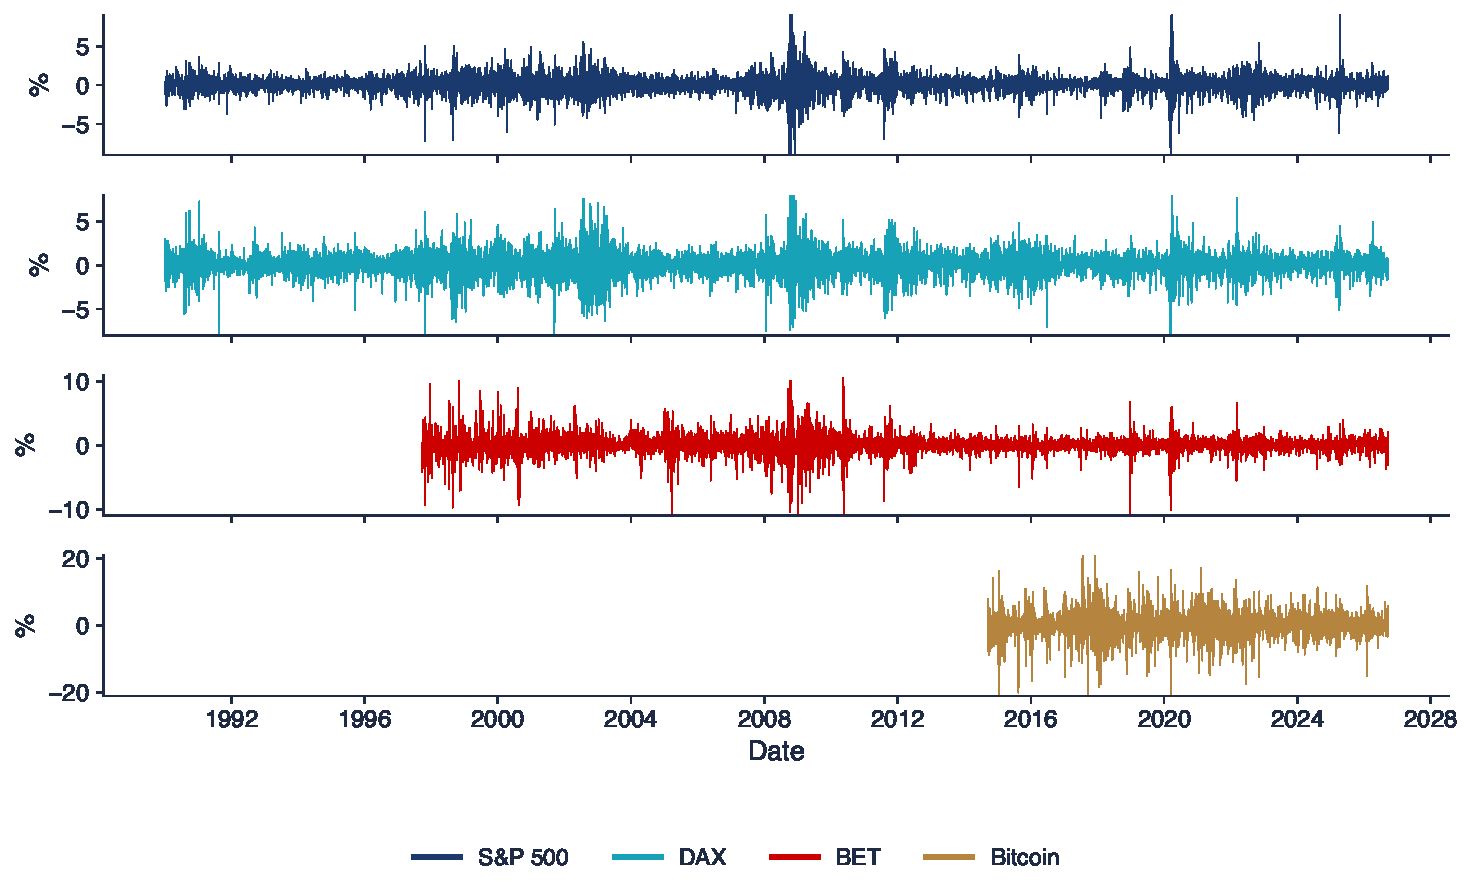
\includegraphics[width=0.97\textwidth,height=0.66\textheight,keepaspectratio]{sfm_ch8_returns_bursts.pdf}
\end{center}
\vspace{-0.25cm}
\begin{itemize}
    \item Daily log returns in \%: S\&P 500 and DAX since 1990, BET since 1997, Bitcoin since 2014; last day 18 September 2026
    \item Quiet years alternate with turbulent months in all four series
\end{itemize}
\sfmquantlet{Ch_08}{SFM_ch8_returns_volatility}
\end{frame}

\begin{frame}{Interpretation: Volatility in Four Markets}
\itemsize{\footnotesize}
\begin{center}
\footnotesize
\begin{tabular}{lrrrr}
\toprule
& \textbf{Annual volatility} & \textbf{Largest daily move} & \textbf{Date} & \textbf{Excess kurtosis} \\
\midrule
S\&P 500 & 18.0\% & ${-12.8}\%$ & 16 March 2020 & 10.9 \\
DAX & 21.8\% & ${-13.1}\%$ & 12 March 2020 & 6.0 \\
BET & 23.4\% & ${-13.1}\%$ & 7 January 2009 & 9.9 \\
Bitcoin & 66.6\% & ${-46.5}\%$ & 12 March 2020 & 12.0 \\
\bottomrule
\end{tabular}
\end{center}
\begin{itemize}
    \item Bitcoin is about 20\% more volatile per year than its daily figure suggests if one wrongly uses $\sqrt{252}$: it trades 365 days a year
    \item The largest moves are 8 to 13 standard deviations: practically impossible under the Normal distribution (\sfmchlink{https://danpele.github.io/SFM/EN/Courses/chapter2_classical_distributions_stylised_facts.pdf}{Chapter 2})
    \item Excess kurtosis far above 0 (the Normal value): heavy tails; Section 6 shows that clustering is one cause
\end{itemize}\sfmquantlet{Ch_08}{SFM_ch8_returns_volatility}
\end{frame}

\begin{frame}{Volatility Is Latent}
\itemsize{\small}
\begin{itemize}
    \item Model: $r_t = \mu + \sigma_t z_t$, with $z_t$ i.i.d., mean 0, variance 1
    \begin{itemize}
        \item $\sigma_t$ is the \textbf{conditional volatility}: $\sigma_t^2 = \mathrm{Var}(r_t \mid \mathcal{F}_{t-1})$, with $\mathcal{F}_{t-1}$ the information at the close of day $t-1$
        \item the \textbf{unconditional volatility} $\sigma = \sqrt{\mathrm{Var}(r_t)}$ is its long-run average level
    \end{itemize}
    \item \textbf{Latent}: we never observe $\sigma_t$, only one return per day
    \begin{itemize}
        \item $r_t^2$ is an unbiased but very noisy measure of $\sigma_t^2$ (with $\mu = 0$): $E[r_t^2 \mid \mathcal{F}_{t-1}] = \sigma_t^2$
        \item a quiet day can happen in a turbulent period, and the other way round
    \end{itemize}
    \item Three ways to get more information about $\sigma_t$
    \begin{itemize}
        \item average many days (historical volatility, EWMA); use the whole daily path (high and low prices); use intraday prices (realised volatility)
    \end{itemize}
\end{itemize}
\end{frame}

\begin{frame}{Worked Example: Annualising Volatility}
\itemsize{\small}
\begin{itemize}
    \item S\&P 500 since 1990: daily standard deviation $\hat\sigma = 1.13\%$, $a = 252$ observations per year
    \begin{itemize}
        \item $\hat\sigma_{\text{year}} = 1.13 \times \sqrt{252} = 1.13 \times 15.87 = 18.0\%$
    \end{itemize}
    \item Bitcoin since 2014: $\hat\sigma = 3.49\%$ per day, 7 days a week
    \begin{itemize}
        \item correct: $3.49 \times \sqrt{365} = 3.49 \times 19.11 = 66.6\%$
        \item wrong, with the equity convention: $3.49 \times \sqrt{252} = 55.3\%$
    \end{itemize}
    \item Comparing assets: annualise each with its own calendar, then compare
\end{itemize}
\end{frame}

\begin{frame}{Recap: What Is Volatility?}
\itemsize{\small}
\begin{itemize}
    \item Volatility = standard deviation of returns; annualise with $\sqrt{a}$, $a$ the actual number of observations per year
    \item Conditional volatility $\sigma_t$ changes over time and is never observed: we can only estimate it
    \item All markets show quiet and turbulent periods
\end{itemize}
\end{frame}


%=============================================================================
\section{Historical Volatility and the Choice of the Window}
%=============================================================================

\begin{frame}{Historical (Rolling) Volatility}
\itemsize{\small}
\begin{itemize}
    \item \textbf{Historical volatility} on a window of the last $n$ days:
    \begin{itemize}
        \item $\hat\sigma_t = \sqrt{\dfrac{1}{n-1}\sum_{j=0}^{n-1}(r_{t-j} - \bar r_t)^2}$, with $\bar r_t$ the mean of the same $n$ returns
        \item \textbf{rolling window}: each day the newest return enters and the oldest leaves
    \end{itemize}
    \item Zero-mean version: $\hat\sigma_t^2 = \frac{1}{n}\sum_{j=0}^{n-1} r_{t-j}^2$
    \begin{itemize}
        \item for daily data the mean is tiny compared with $\sigma$ ($0.03\%$ against $1.13\%$ for the S\&P 500); setting it to 0 removes a noisy estimate
    \end{itemize}
    \item Usual windows: $n = 21$ (a month), $63$ (a quarter), $252$ (a year) of trading days
    \begin{itemize}
        \item each $\hat\sigma_t$ is annualised with $\sqrt{a}$ and plotted at the last day of its window
    \end{itemize}
\end{itemize}
\end{frame}

\begin{frame}{S\&P 500: Three Windows, Three Answers}
\itemsize{\footnotesize}
\begin{center}
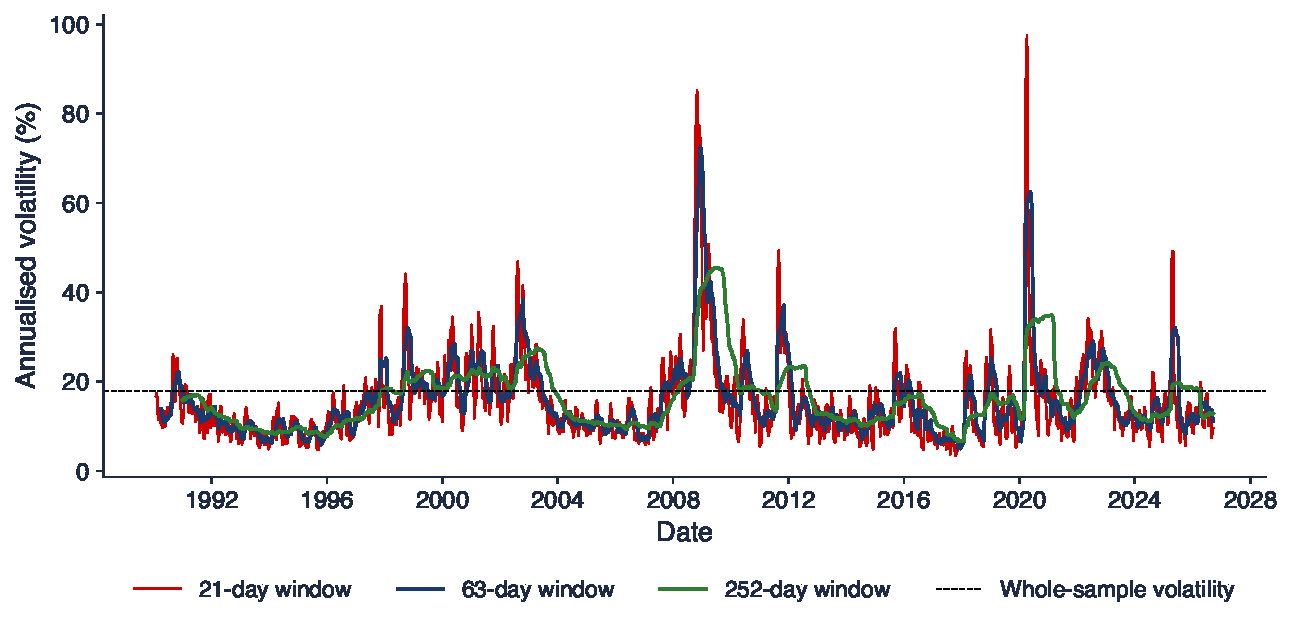
\includegraphics[width=0.97\textwidth,height=0.56\textheight,keepaspectratio]{sfm_ch8_rolling_windows.pdf}
\end{center}
\vspace{-0.25cm}
\begin{itemize}
    \item Rolling volatility of the S\&P 500, annualised; dashed line: the whole-sample volatility, 18.0\%
    \item \textbf{Question for the room}: which window would you trust on the day after a crash?
\end{itemize}
\sfmquantlet{Ch_08}{SFM_ch8_returns_volatility}
\end{frame}

\begin{frame}{Interpretation: the Window Trade-Off}
\itemsize{\small}
\begin{itemize}
    \item Short window ($n = 21$): reacts fast, but is noisy
    \begin{itemize}
        \item maximum 97.5\% on 6 April 2020; the typical daily change of $\ln\hat\sigma_t$ is 6.7\%
    \end{itemize}
    \item Long window ($n = 252$): smooth, but slow
    \begin{itemize}
        \item maximum only 45.6\%, reached on 15 July 2009, months after the peak of the 2008 crisis; daily change 0.8\%
    \end{itemize}
    \item \textbf{Answer}: a short window, or EWMA (next section), because a long window still averages the calm days before the crash
    \begin{itemize}
        \item for capital planning, a long window is preferred: it changes slowly
    \end{itemize}
    \item At the end of the sample: 9.6\% (21 days), 11.1\% (63 days), 12.9\% (252 days)
\end{itemize}\sfmquantlet{Ch_08}{SFM_ch8_returns_volatility}
\end{frame}

\begin{frame}{How Precise Is a Sample Volatility?}
\itemsize{\small}
\begin{itemize}
    \item With $n$ i.i.d.\ Normal returns, the relative standard error of $\hat\sigma$ is $\mathrm{SE}(\hat\sigma)/\sigma \approx 1/\sqrt{2n}$
    \begin{itemize}
        \item $n = 21$: 15\%; $n = 63$: 9\%; $n = 252$: 4\%
    \end{itemize}
    \item With heavy tails (kurtosis $\kappa$): $\mathrm{SE}(\hat\sigma)/\sigma \approx \sqrt{(\kappa - 1)/(4n)}$ (delta method)
    \begin{itemize}
        \item S\&P 500: $\kappa = 13.9$, so $n = 21$: 39\%; $n = 252$: 11\%
        \item for $\kappa = 3$ (Normal) the two formulas coincide
    \end{itemize}
    \item \textbf{Worked example}: the last 21-day volatility of the S\&P 500 is 9.6\%
    \begin{itemize}
        \item approximate 95\% interval, Normal returns: $[6.7\%; 12.5\%]$; with the observed kurtosis: $[2.2\%; 17.0\%]$
    \end{itemize}
\end{itemize}
\end{frame}

\begin{frame}{Recap: Historical Volatility}
\itemsize{\small}
\begin{itemize}
    \item Rolling standard deviation on $n$ days; daily data: the mean can be set to zero
    \item Short windows react fast but are noisy; long windows are smooth but slow
    \item A 21-day volatility is uncertain by $\pm$15\% or more: one decimal is already too much precision
\end{itemize}
\end{frame}


%=============================================================================
\section{EWMA and RiskMetrics}
%=============================================================================

\begin{frame}{1994: RiskMetrics Makes Volatility a Daily Number}
\itemsize{\small}
\begin{columns}[T]
\begin{column}{0.56\textwidth}
\begin{itemize}
    \item J.P. Morgan launched RiskMetrics in October 1994 and published its methods and data free of charge \refRM
    \begin{itemize}
        \item goal: one common yardstick for market risk across banks
        \item volatilities and correlations of more than 480 series, updated every day
    \end{itemize}
    \item The method: an exponentially weighted moving average (EWMA) of squared returns
    \begin{itemize}
        \item one parameter, the \textbf{decay factor} $\lambda$: $0.94$ for daily forecasts, $0.97$ for monthly ones
        \item for each series, $\lambda$ minimises the root mean squared error of its variance forecasts; 0.94 is the weighted average over all series
    \end{itemize}
\end{itemize}
\end{column}
\begin{column}{0.40\textwidth}
\centering
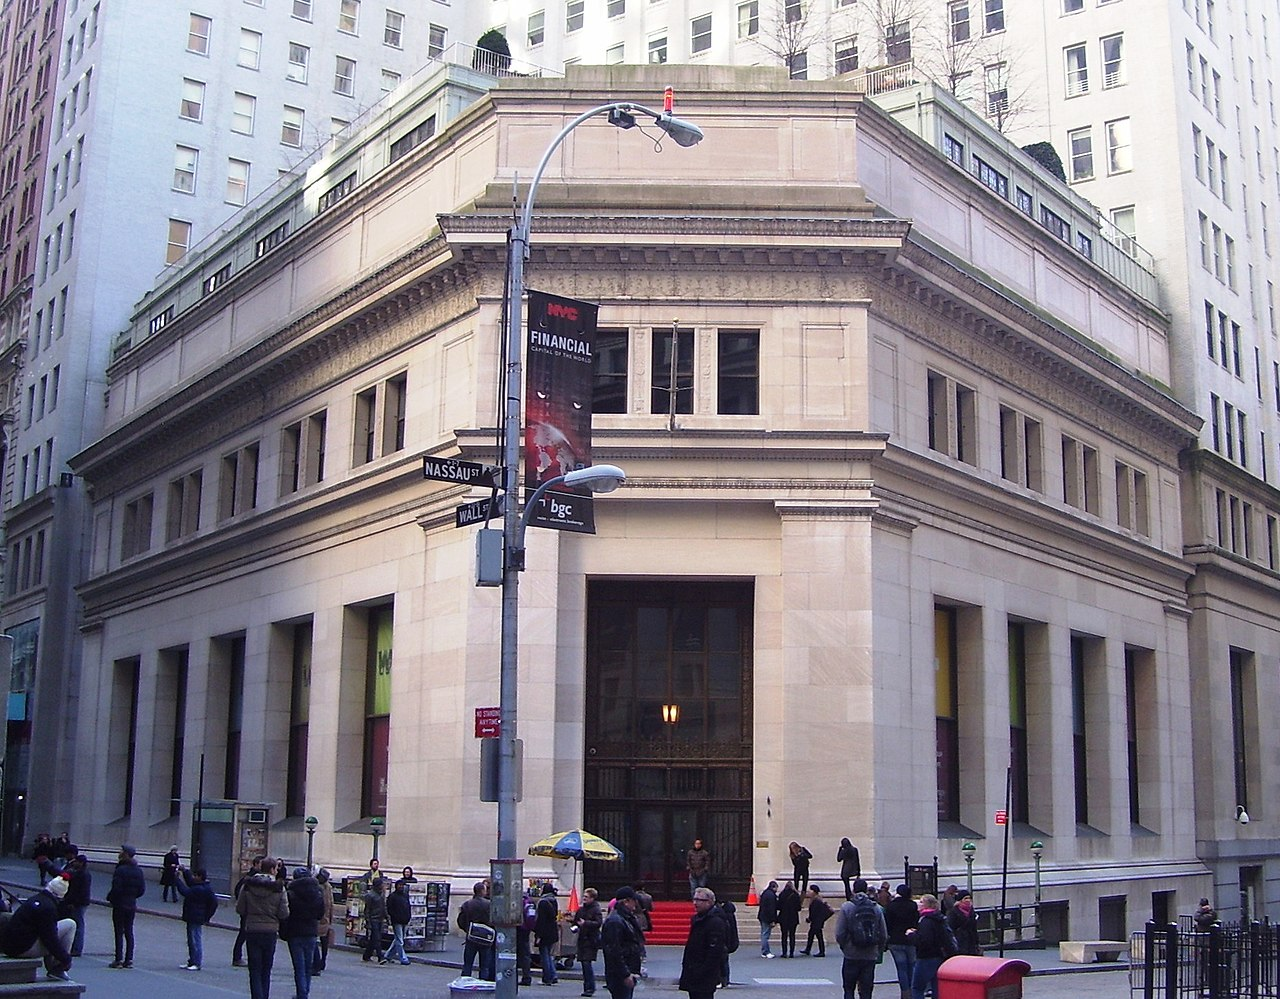
\includegraphics[height=0.38\textheight]{ch8_jpmorgan_23wall.jpg}\\[1mm]
\imgcap{The J.P. Morgan building at 23 Wall Street, New York}
\imgcredit{https://commons.wikimedia.org/wiki/File:J._P._Morgan_\%26_Company_Building_23_Wall_Street.jpg}{Photo: Beyond My Ken (2012); CC BY-SA 4.0; Wikimedia Commons}
\end{column}
\end{columns}
\end{frame}

\begin{frame}{The EWMA Estimator}
\itemsize{\small}
\begin{itemize}
    \item \textbf{EWMA} recursion (zero mean): $\sigma_t^2 = \lambda\,\sigma_{t-1}^2 + (1-\lambda)\,r_{t-1}^2$, \ $0 < \lambda < 1$
    \begin{itemize}
        \item $\sigma_t^2$ uses returns up to day $t-1$: it is the forecast for day $t$
        \item start: $\sigma_1^2$ = the mean of the first squared returns; its effect fades after a few months
    \end{itemize}
    \item Unrolling the recursion: $\sigma_t^2 = (1-\lambda)\sum_{j \ge 1}\lambda^{j-1} r_{t-j}^2$
    \begin{itemize}
        \item weights $(1-\lambda)\lambda^{j-1}$ decline geometrically and sum to 1
        \item \textbf{half-life}: the lag at which the weight halves, $\ln 0.5/\ln\lambda$
    \end{itemize}
    \item A rolling window gives weight $1/n$ to each of the last $n$ days and 0 to all older days
\end{itemize}
\end{frame}

\begin{frame}{EWMA Weights against a Rolling Window}
\itemsize{\footnotesize}
\begin{center}
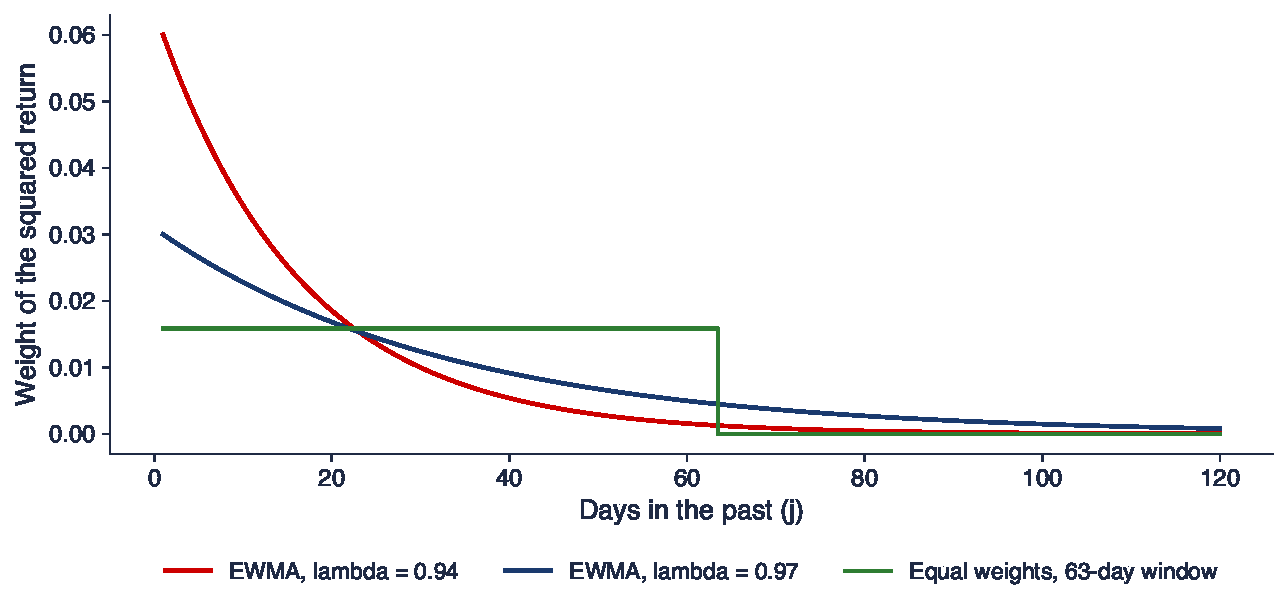
\includegraphics[width=0.97\textwidth,height=0.54\textheight,keepaspectratio]{sfm_ch8_ewma_weights.pdf}
\end{center}
\vspace{-0.25cm}
\begin{itemize}
    \item $\lambda = 0.94$: half-life 11.2 days, mean lag $1/(1-\lambda) = 16.7$ days, 99\% of the weight in the last 74 days
    \item $\lambda = 0.97$: half-life 22.8 days, 99\% of the weight in the last 151 days
\end{itemize}
\sfmquantlet{Ch_08}{SFM_ch8_ewma}
\end{frame}

\begin{frame}{Worked Example: One EWMA Update}
\itemsize{\small}
\begin{itemize}
    \item Yesterday's EWMA variance: $\sigma_{t-1}^2 = 1.00$ (\%$^2$), a daily volatility of 1\%; yesterday's return: $r_{t-1} = -3\%$
    \begin{itemize}
        \item step 1: $\lambda\sigma_{t-1}^2 = 0.94 \times 1.00 = 0.94$
        \item step 2: $(1-\lambda)r_{t-1}^2 = 0.06 \times 9 = 0.54$
        \item step 3: $\sigma_t^2 = 0.94 + 0.54 = 1.48$, so $\sigma_t = 1.22\%$ per day, $1.22 \times \sqrt{252} = 19.3\%$ per year
    \end{itemize}
    \item If today is quiet ($r_t = 0$): $\sigma_{t+1}^2 = 0.94 \times 1.48 = 1.39$
    \begin{itemize}
        \item the shock fades by 6\% per day; it never drops out abruptly
    \end{itemize}
    \item A 63-day window would add $9/63 = 0.14$ to the variance today and remove this contribution at once, 63 days later
\end{itemize}
\end{frame}

\begin{frame}{The Ghost Effect: March--June 2020}
\itemsize{\footnotesize}
\begin{center}
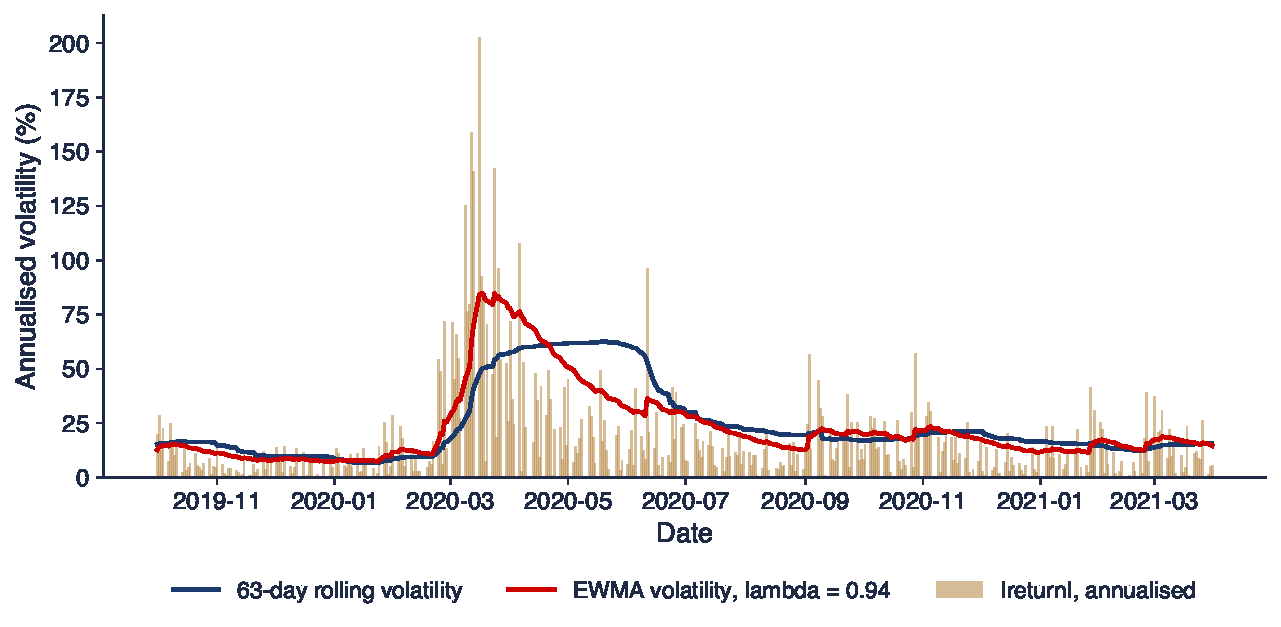
\includegraphics[width=0.97\textwidth,height=0.54\textheight,keepaspectratio]{sfm_ch8_ghost.pdf}
\end{center}
\vspace{-0.25cm}
\begin{itemize}
    \item S\&P 500: 63-day rolling volatility and EWMA volatility ($\lambda = 0.94$), annualised; bars: $|r_t|$ on the same annual scale
    \item \textbf{Question for the room}: why does the blue line fall sharply in mid-June 2020, on a calm day?
\end{itemize}
\sfmquantlet{Ch_08}{SFM_ch8_ewma}
\end{frame}

\begin{frame}{Interpretation: Ghosts and Fading Memory}
\itemsize{\small}
\begin{itemize}
    \item \textbf{Answer}: on 15 June 2020 the return of 16 March 2020 ($-12.8\%$) left the 63-day window
    \begin{itemize}
        \item the rolling volatility fell from 50.4\% to 43.0\% in one day, with no news at all
        \item this artefact is the \textbf{ghost effect}: an old shock leaves the window abruptly
    \end{itemize}
    \item EWMA reacts faster and forgets smoothly
    \begin{itemize}
        \item EWMA peak: 84.8\% on 24 March 2020; 63-day peak: 62.6\% only on 20 May 2020
        \item on the ghost day EWMA changed by only $-0.9$ percentage points
    \end{itemize}
    \item Price of the speed: EWMA is noisier than a long window and has no long-run level to return to
\end{itemize}\sfmquantlet{Ch_08}{SFM_ch8_ewma}
\end{frame}

\begin{frame}{EWMA and GARCH: a Pointer to \sfmchlinkt{https://danpele.github.io/SFM/EN/Courses/chapter9_arch_garch_models.pdf}{Chapter 9}}
\itemsize{\small}
\begin{itemize}
    \item \textbf{ARCH} \refEngle{} and \textbf{GARCH} \refBollerslev: $\sigma_t^2 = \omega + \alpha\, r_{t-1}^2 + \beta\,\sigma_{t-1}^2$
    \begin{itemize}
        \item EWMA is the special case $\omega = 0$, $\alpha = 1 - \lambda$, $\beta = \lambda$, so $\alpha + \beta = 1$ (``integrated'' GARCH, \textbf{IGARCH})
    \end{itemize}
    \item Consequences for forecasts made at day $t$ for day $t + h$
    \begin{itemize}
        \item EWMA: flat, $E_t[\sigma_{t+h}^2] = \sigma_{t+1}^2$ for every $h$: today's level persists for ever
        \item GARCH with $\alpha + \beta < 1$: pulled towards the long-run variance $\omega/(1 - \alpha - \beta)$
    \end{itemize}
    \item \sfmchlink{https://danpele.github.io/SFM/EN/Courses/chapter9_arch_garch_models.pdf}{Chapter 9} estimates $\omega$, $\alpha$, $\beta$ by maximum likelihood; here $\lambda$ is fixed or chosen by a forecast criterion (Section 8)
\end{itemize}
\end{frame}

\begin{frame}{Recap: EWMA and RiskMetrics}
\itemsize{\small}
\begin{itemize}
    \item $\sigma_t^2 = \lambda\sigma_{t-1}^2 + (1-\lambda)r_{t-1}^2$; RiskMetrics: $\lambda = 0.94$ for daily data
    \item Geometric weights: half-life 11.2 days for $\lambda = 0.94$; no ghost effect
    \item EWMA = IGARCH(1,1) without a constant: flat forecasts, no mean reversion
\end{itemize}
\end{frame}


%=============================================================================
\section{Range-Based Estimators}
%=============================================================================

\begin{frame}{Open, High, Low and Close Prices}
\itemsize{\small}
\begin{itemize}
    \item \textbf{OHLC} data: for each day $t$, the open $O_t$, the high $H_t$, the low $L_t$ and the close $C_t$
    \begin{itemize}
        \item the close-to-close return uses 2 prices a day; $H_t$ and $L_t$ carry information about the whole path of the day
    \end{itemize}
    \item Notation (log differences in \%), each from the open of day $t$:
    \begin{itemize}
        \item $u_t = \ln(H_t/O_t)$, $d_t = \ln(L_t/O_t)$, $c_t = \ln(C_t/O_t)$; so $d_t \le 0 \le u_t$ and $d_t \le c_t \le u_t$
        \item \textbf{overnight} return $o_t = \ln(O_t/C_{t-1})$; the daily return is $r_t = o_t + c_t$
        \item the \textbf{range} $u_t - d_t = \ln(H_t/L_t)$
    \end{itemize}
    \item Data: S\&P 500 since 2008, DAX since 2006, Bitcoin since 2014, BVB stocks since 2010; the BET file has closes only
\end{itemize}
\end{frame}

\begin{frame}{One Trading Day: What OHLC Records}
\itemsize{\footnotesize}
\begin{center}
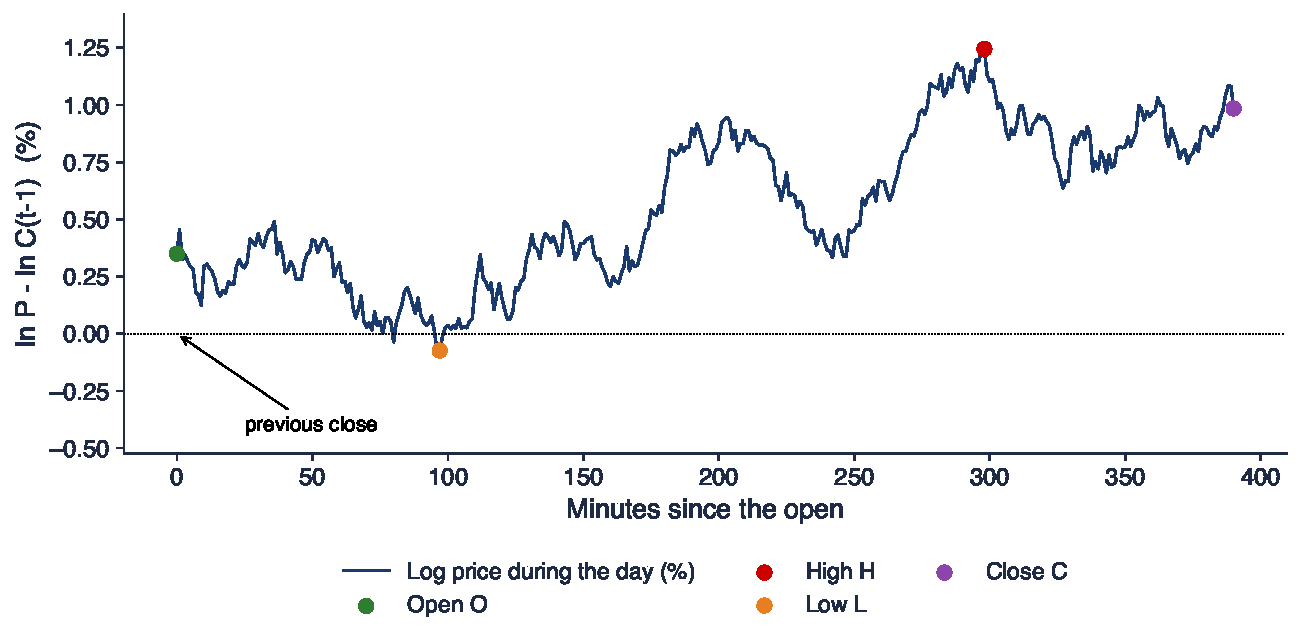
\includegraphics[width=0.97\textwidth,height=0.54\textheight,keepaspectratio]{sfm_ch8_ohlc_path.pdf}
\end{center}
\vspace{-0.25cm}
\begin{itemize}
    \item Simulated log price (Brownian motion, 390 one-minute steps) after an overnight gap of $0.35\%$: the close keeps only the end point; high and low summarise the path
    \item Two days with the same close can have very different ranges, and so very different risk
\end{itemize}
\sfmquantlet{Ch_08}{SFM_ch8_range_estimators}
\end{frame}

\begin{frame}{The Parkinson Estimator (1980)}
\itemsize{\small}
\begin{itemize}
    \item For a Brownian motion with no drift and variance $\sigma^2$ per day: $E[(u_t - d_t)^2] = 4\ln 2\;\sigma^2$ \refParkinson
    \begin{itemize}
        \item one day: $\hat\sigma_{P,t}^2 = \dfrac{(u_t - d_t)^2}{4\ln 2}$; on $n$ days: the mean of these values
        \item $4\ln 2 \approx 2.77$: the range is on average larger than $\sigma$
    \end{itemize}
    \item Assumptions
    \begin{itemize}
        \item continuous trading during the day, so the observed high and low are the true extremes
        \item no drift and no overnight jump: the range only sees the trading session
    \end{itemize}
    \item Much more precise than $r_t^2$: a simulation later in this section measures by how much
    \begin{itemize}
        \item the log range is also used to estimate stochastic volatility models \refABD
    \end{itemize}
\end{itemize}
\end{frame}

\begin{frame}{Garman--Klass (1980) and Rogers--Satchell (1991)}
\itemsize{\small}
\begin{itemize}
    \item \textbf{Garman--Klass} \refGK: adds the open-to-close return
    \begin{itemize}
        \item $\hat\sigma_{GK,t}^2 = 0.5\,(u_t - d_t)^2 - (2\ln 2 - 1)\,c_t^2$
        \item the weights make the estimator unbiased and nearly of minimum variance among such quadratic forms, under no drift
    \end{itemize}
    \item \textbf{Rogers--Satchell} \refRS: unbiased for any drift $\mu$
    \begin{itemize}
        \item $\hat\sigma_{RS,t}^2 = u_t(u_t - c_t) + d_t(d_t - c_t)$
        \item useful for assets with a strong trend over the window (for example, Bitcoin in a strong rally)
    \end{itemize}
    \item Both still ignore the overnight return $o_t$: they measure the variance of the trading session only
\end{itemize}
\end{frame}

\begin{frame}{Yang--Zhang (2000): Adding the Night}
\itemsize{\small}
\begin{itemize}
    \item On a window of $n$ days \refYZ:
    \begin{itemize}
        \item $\hat\sigma_{YZ}^2 = \hat\sigma_O^2 + k\,\hat\sigma_C^2 + (1-k)\,\hat\sigma_{RS}^2$, \quad $k = \dfrac{0.34}{1.34 + (n+1)/(n-1)}$
        \item $\hat\sigma_O^2$, $\hat\sigma_C^2$: sample variances of the overnight returns $o_t$ and of the open-to-close returns $c_t$; $\hat\sigma_{RS}^2$: the mean Rogers--Satchell term
    \end{itemize}
    \item Properties
    \begin{itemize}
        \item unbiased with drift and with opening jumps; $k$ minimises the variance of the estimator
        \item $n = 21$: $k = 0.34/(1.34 + 22/20) = 0.34/2.44 = 0.14$
    \end{itemize}
    \item Needs a window of $n \ge 2$ days (sample variances); Parkinson, Garman--Klass and Rogers--Satchell also work for a single day
\end{itemize}
\end{frame}

\begin{frame}{Worked Example: S\&P 500 on 16 March 2020}
\itemsize{\small}
\begin{itemize}
    \item Previous close 2\,711; open 2\,509, high 2\,563, low 2\,381, close 2\,386
    \begin{itemize}
        \item $o = -7.76$, $u = 2.14$, $d = -5.22$, $c = -5.00$ (in \%); close-to-close $r = o + c = -12.77$
    \end{itemize}
    \item One-day variance estimates (\%$^2$)
    \begin{itemize}
        \item close-to-close: $r^2 = 163.0$
        \item Parkinson: $(7.37)^2/2.773 = 19.6$; Garman--Klass: 17.5; Rogers--Satchell: 16.5
        \item overnight part $o^2 = 60.2$; overnight plus Rogers--Satchell: 76.7
    \end{itemize}
    \item Most of the fall happened overnight, before the open: estimators that ignore $o_t$ miss most of the risk of this day
\end{itemize}\sfmquantlet{Ch_08}{SFM_ch8_range_estimators}
\end{frame}

\begin{frame}{Efficiency by Simulation}
\itemsize{\footnotesize}
\begin{center}
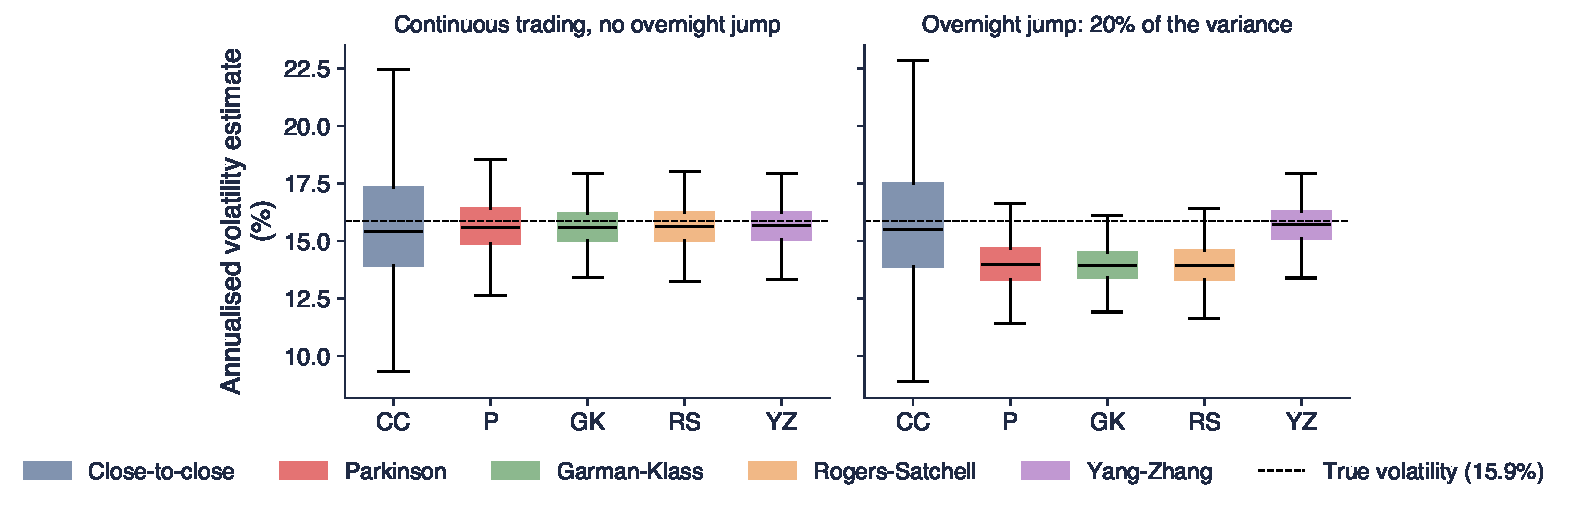
\includegraphics[width=0.97\textwidth,height=0.52\textheight,keepaspectratio]{sfm_ch8_efficiency.pdf}
\end{center}
\vspace{-0.25cm}
\begin{itemize}
    \item 1000 windows of 21 days; true volatility $1\%$ per day ($15.9\%$ per year); intraday Brownian motion on 4680 steps (one every 5 seconds)
    \item \textbf{Efficiency} of an estimator: $\mathrm{Var}(\hat\sigma^2_{CC})/\mathrm{Var}(\hat\sigma^2)$, with CC the close-to-close estimator; right panel: 20\% of the daily variance comes overnight
\end{itemize}
\sfmquantlet{Ch_08}{SFM_ch8_range_efficiency}
\end{frame}

\begin{frame}{Interpretation: Precision Is Not Accuracy}
\itemsize{\footnotesize}
\begin{center}
\footnotesize
\begin{tabular}{lrrrrr}
\toprule
& \textbf{CC} & \textbf{Parkinson} & \textbf{GK} & \textbf{RS} & \textbf{YZ} \\
\midrule
Efficiency, continuous trading & 1.0 & 5.4 & 9.3 & 7.6 & 8.5 \\
Bias (\%), continuous trading & ${0}$ & ${-2}$ & ${-3}$ & ${-3}$ & ${-2}$ \\
Bias (\%), overnight jump & ${1}$ & ${-22}$ & ${-22}$ & ${-22}$ & ${-2}$ \\
MSE ratio, overnight jump & 1.0 & 1.8 & 1.8 & 1.8 & 9.0 \\
Bias (\%), 26 prices a day & ${0}$ & ${-23}$ & ${-32}$ & ${-32}$ & ${-28}$ \\
\bottomrule
\end{tabular}
\end{center}
\begin{itemize}
    \item With continuous trading, range estimators are 5 to 9 times more efficient: one month of ranges carries as much information as 5 to 9 months of closes
    \item With an overnight jump, Parkinson, GK and RS miss the night (bias about $-22\%$); only YZ stays unbiased; \textbf{MSE} (mean squared error) ratio = $\mathrm{MSE}(CC)/\mathrm{MSE}$
    \item With few trades the observed range is too small: all range estimators underestimate (thin markets) \refMolnar
\end{itemize}\sfmquantlet{Ch_08}{SFM_ch8_range_efficiency}
\end{frame}

\begin{frame}{Real Data: Five Estimators, Five Assets}
\itemsize{\footnotesize}
\begin{center}
\footnotesize
\begin{tabular}{lrrrrrrrr}
\toprule
& \textbf{Since} & \textbf{CC} & \textbf{P} & \textbf{GK} & \textbf{RS} & \textbf{YZ} & \textbf{Night share} & $\mathrm{corr}(o, c)$ \\
\midrule
S\&P 500 & 2008 & 19.9 & 15.4 & 14.6 & 14.4 & 16.3 & 13\% & ${0.22}$ \\
DAX & 2006 & 20.9 & 16.7 & 16.6 & 16.6 & 20.3 & 31\% & ${0.02}$ \\
Bitcoin & 2014 & 66.6 & 63.5 & 62.4 & 62.5 & 63.2 & 0\% & ${0.02}$ \\
TLV & 2010 & 26.6 & 21.5 & 20.6 & 21.0 & 25.6 & 26\% & ${-0.08}$ \\
SNP & 2010 & 24.5 & 21.4 & 20.8 & 21.4 & 25.8 & 27\% & ${-0.20}$ \\
\bottomrule
\end{tabular}
\end{center}
\begin{itemize}
    \item Annualised volatility (\%) on the whole OHLC sample; P = Parkinson; night share $= \hat\sigma_O^2/(\hat\sigma_O^2 + \hat\sigma_C^2)$
    \item Stocks: open, high and low adjusted with the same factor as the close; days without trades removed
\end{itemize}\sfmquantlet{Ch_08}{SFM_ch8_range_estimators}
\end{frame}

\begin{frame}{Interpretation: Why the Estimators Disagree}
\itemsize{\small}
\begin{itemize}
    \item Bitcoin trades 24 hours a day: the night share is almost 0, and all five estimators agree within a few points
    \begin{itemize}
        \item the remaining gap: the daily path is observed in discrete trades, not continuously
    \end{itemize}
    \item DAX and the BVB stocks: a quarter to a third of the variance comes overnight
    \begin{itemize}
        \item Parkinson, GK and RS are far below CC; YZ, which adds the night, is close to CC
    \end{itemize}
    \item S\&P 500: even YZ (16.3\%) stays below CC (19.9\%)
    \begin{itemize}
        \item overnight and open-to-close returns are positively correlated (0.22); a likely reason: the index open uses stale prices of stocks that have not traded yet
        \item $\mathrm{Var}(r) = \mathrm{Var}(o) + \mathrm{Var}(c) + 2\,\mathrm{Cov}(o, c)$: no range estimator sees the covariance term
    \end{itemize}
    \item Lesson: check the assumptions on the data before trusting an efficiency gain
\end{itemize}\sfmquantlet{Ch_08}{SFM_ch8_range_estimators}
\end{frame}

\begin{frame}{S\&P 500: Rolling 21-Day Estimates since 2019}
\itemsize{\footnotesize}
\begin{center}
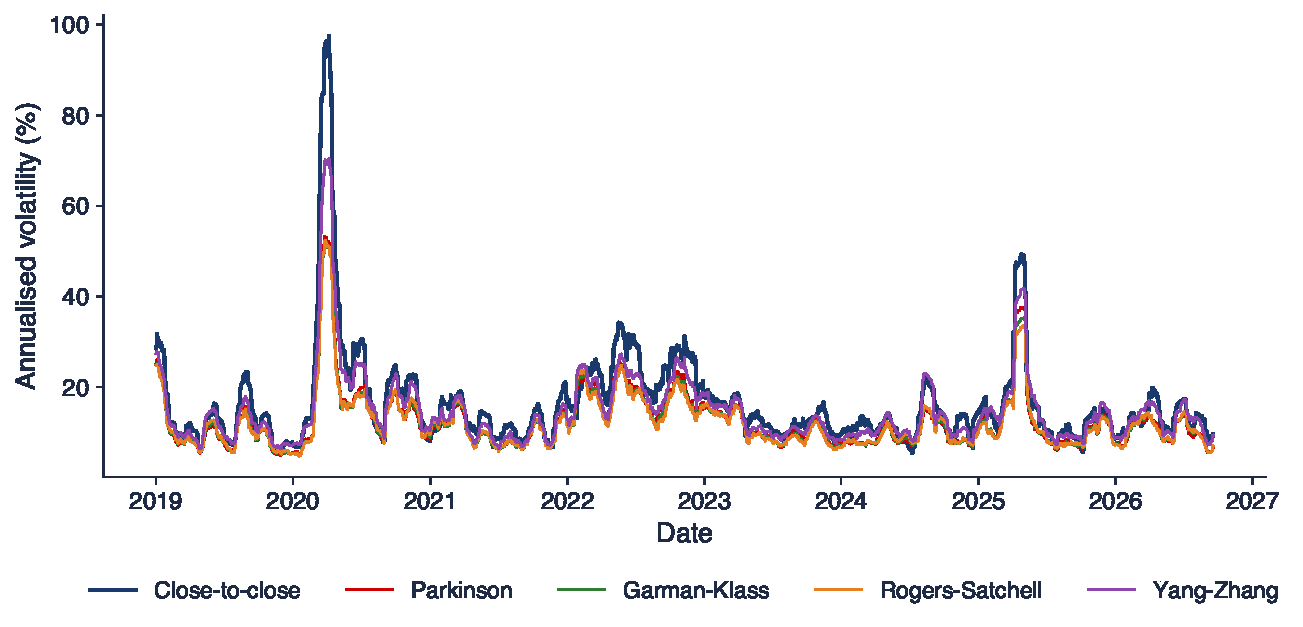
\includegraphics[width=0.97\textwidth,height=0.54\textheight,keepaspectratio]{sfm_ch8_range_rolling.pdf}
\end{center}
\vspace{-0.25cm}
\begin{itemize}
    \item Annualised 21-day volatility by the five estimators; means since 2019: CC 16.3\%, Parkinson 12.5\%, YZ 14.7\%
    \item The range-based lines are smoother: the typical daily change of the log estimate is 4.3\% for Parkinson and 4.2\% for YZ, against 7.1\% for CC
\end{itemize}
\sfmquantlet{Ch_08}{SFM_ch8_range_estimators}
\end{frame}

\begin{frame}{Recap: Range-Based Estimators}
\itemsize{\small}
\begin{itemize}
    \item Parkinson uses the range, Garman--Klass adds the open-to-close return, Rogers--Satchell allows a drift, Yang--Zhang adds the night
    \item In theory 5 to 9 times more efficient than close-to-close; in practice biased down by overnight jumps and discrete trading
    \item Choose Yang--Zhang for markets that close at night; any range estimator for 24-hour markets
\end{itemize}
\end{frame}


%=============================================================================
\section{Realised Volatility}
%=============================================================================

\begin{frame}{Realised Variance from Intraday Returns}
\itemsize{\small}
\begin{itemize}
    \item Split day $t$ into $M$ intervals (for example $M = 78$ five-minute returns $r_{t,i}$ in a 6.5-hour session)
    \begin{itemize}
        \item \textbf{realised variance} $\mathrm{RV}_t = \sum_{i=1}^{M} r_{t,i}^2$; \textbf{realised volatility} $= \sqrt{\mathrm{RV}_t}$
        \item as $M \to \infty$, $\mathrm{RV}_t$ converges to the \textbf{integrated variance} of day $t$, the true variance of the day \refABDL, \refBNS
    \end{itemize}
    \item Volatility becomes almost observable: a nearly error-free measure for each day
    \begin{itemize}
        \item used to evaluate forecasts (Section 8) and to forecast volatility directly, for example with the HAR model \refCorsi
        \item high-frequency Bitcoin prices and daily risk: \refPeleB
    \end{itemize}
    \item Our course data are daily; the next two slides use simulated one-minute prices to show how RV behaves
\end{itemize}
\end{frame}

\begin{frame}{Simulated Example: RV Tracks the True Volatility}
\itemsize{\footnotesize}
\begin{center}
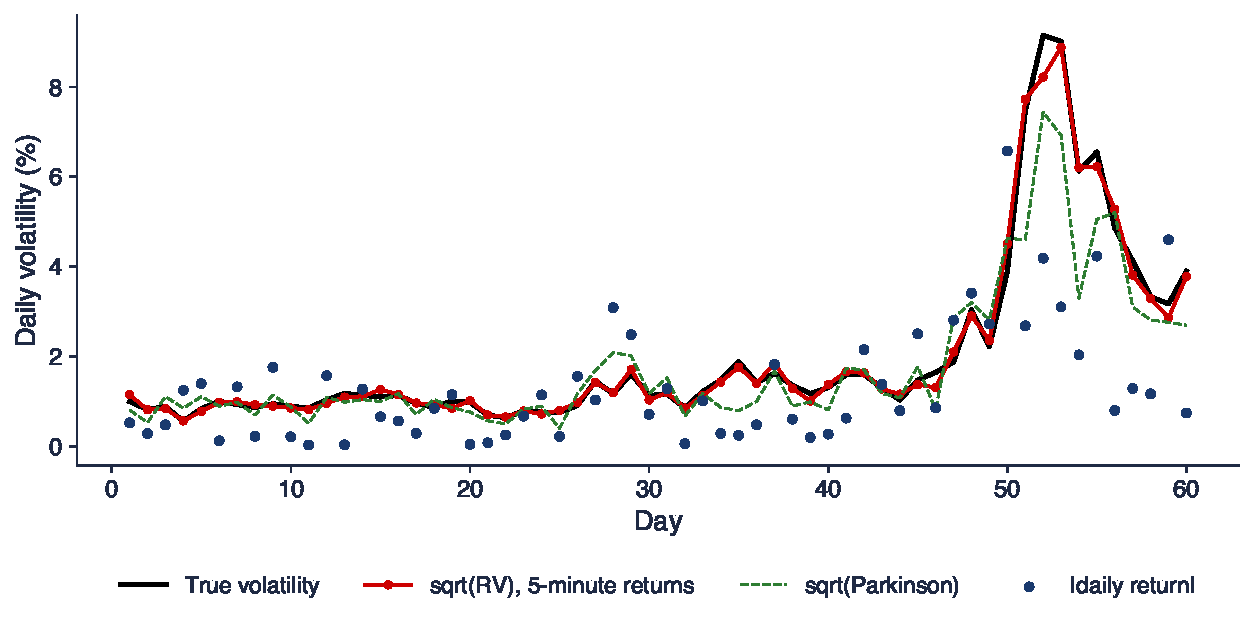
\includegraphics[width=0.97\textwidth,height=0.52\textheight,keepaspectratio]{sfm_ch8_realised.pdf}
\end{center}
\vspace{-0.25cm}
\begin{itemize}
    \item 60 simulated days of 390 one-minute returns; the daily volatility follows a log AR(1) process (persistence $0.9$)
    \item Mean absolute relative error: 5-minute RV 6\%, Parkinson 23\%, $|r_t|$ 58\%; correlation with the truth: 0.995, 0.94 and 0.59
\end{itemize}
\sfmquantlet{Ch_08}{SFM_ch8_realised_volatility}
\end{frame}

\begin{frame}{Microstructure Noise and the Signature Plot}
\itemsize{\footnotesize}
\begin{center}
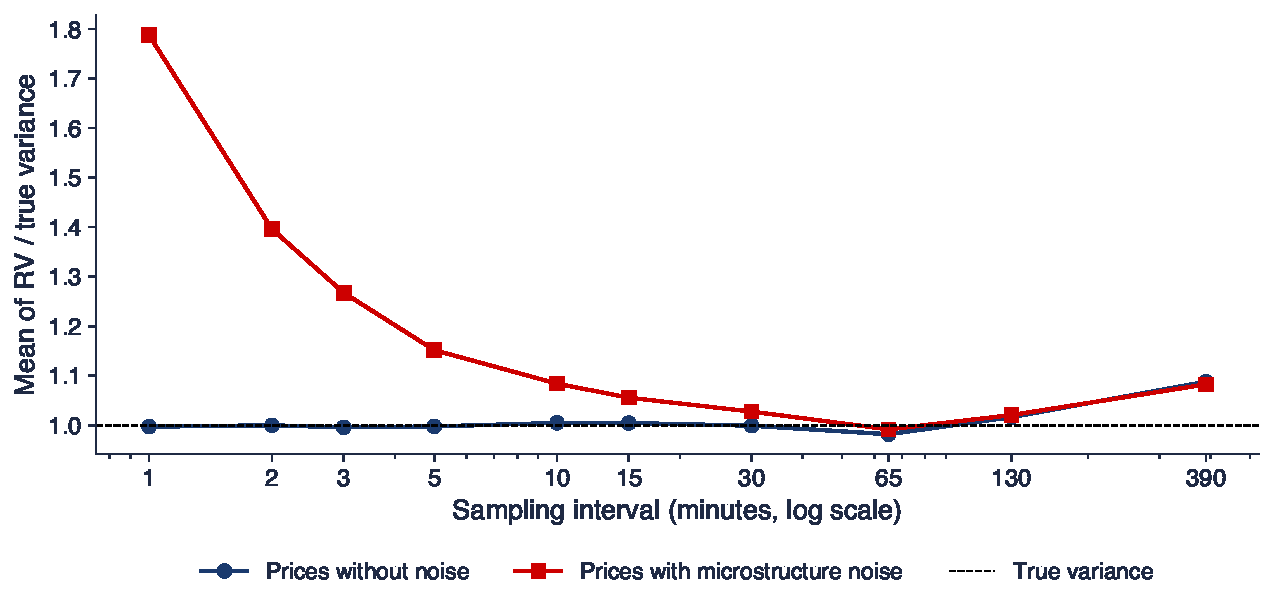
\includegraphics[width=0.97\textwidth,height=0.46\textheight,keepaspectratio]{sfm_ch8_signature.pdf}
\end{center}
\vspace{-0.25cm}
\begin{itemize}
    \item Observed prices = true prices + \textbf{microstructure noise} (bid--ask bounce, price ticks), here with sd $0.025\%$; each squared return then adds $2\times$ the noise variance
    \item With noise, one-minute RV overstates the variance by a factor of 1.79; at 5 minutes: 1.15; the \textbf{signature plot} shows RV against the sampling interval
    \item In practice, 5-minute RV is hard to beat \refLPS
\end{itemize}
\sfmquantlet{Ch_08}{SFM_ch8_realised_volatility}
\end{frame}

\begin{frame}{Recap: Realised Volatility}
\itemsize{\small}
\begin{itemize}
    \item $\mathrm{RV}_t = \sum_i r_{t,i}^2$ estimates the variance of one day almost without error
    \item Too frequent sampling picks up microstructure noise; 5 minutes is the usual compromise
    \item Ranking of daily measures: RV $>$ range estimators $>$ squared daily return
\end{itemize}
\end{frame}


%=============================================================================
\section{Volatility Clustering}
%=============================================================================

\begin{frame}{1982: Engle and the ARCH Model}
\itemsize{\small}
\begin{columns}[T]
\begin{column}{0.60\textwidth}
\begin{itemize}
    \item \textbf{Volatility clustering}: periods of large absolute returns alternate with periods of small ones \refMandelbrot, \refCont
    \begin{itemize}
        \item returns are almost uncorrelated (\sfmchlink{https://danpele.github.io/SFM/EN/Courses/chapter7_efficient_markets_random_walk_vr.pdf}{Chapter 7}), but $|r_t|$ and $r_t^2$ are strongly autocorrelated
    \end{itemize}
    \item Robert F. Engle \refEngle: the variance of today depends on yesterday's squared shocks: \textbf{ARCH}
    \begin{itemize}
        \item the first model in which $\sigma_t$ changes over time in a predictable way
        \item Nobel Prize in Economic Sciences 2003, shared with Clive Granger \refNobel; Engle's Nobel lecture: \refEngleN
    \end{itemize}
    \item This section: tests for clustering; \sfmchlink{https://danpele.github.io/SFM/EN/Courses/chapter9_arch_garch_models.pdf}{Chapter 9}: the models
\end{itemize}
\end{column}
\begin{column}{0.36\textwidth}
\centering

\includegraphics[height=0.40\textheight]{ch8_engle_2017.png}\\[1mm]
\imgcap{Robert F. Engle (b. 1942), Santiago, 2017}
\imgcredit{https://commons.wikimedia.org/wiki/File:Robert_Engle_SantiagoWEAI2017.png}{Photo: Econterms (2017); CC BY-SA 4.0; Wikimedia Commons}
\end{column}
\end{columns}
\end{frame}

\begin{frame}{The Sign Is Unpredictable, the Size Is Not}
\itemsize{\footnotesize}
\begin{center}
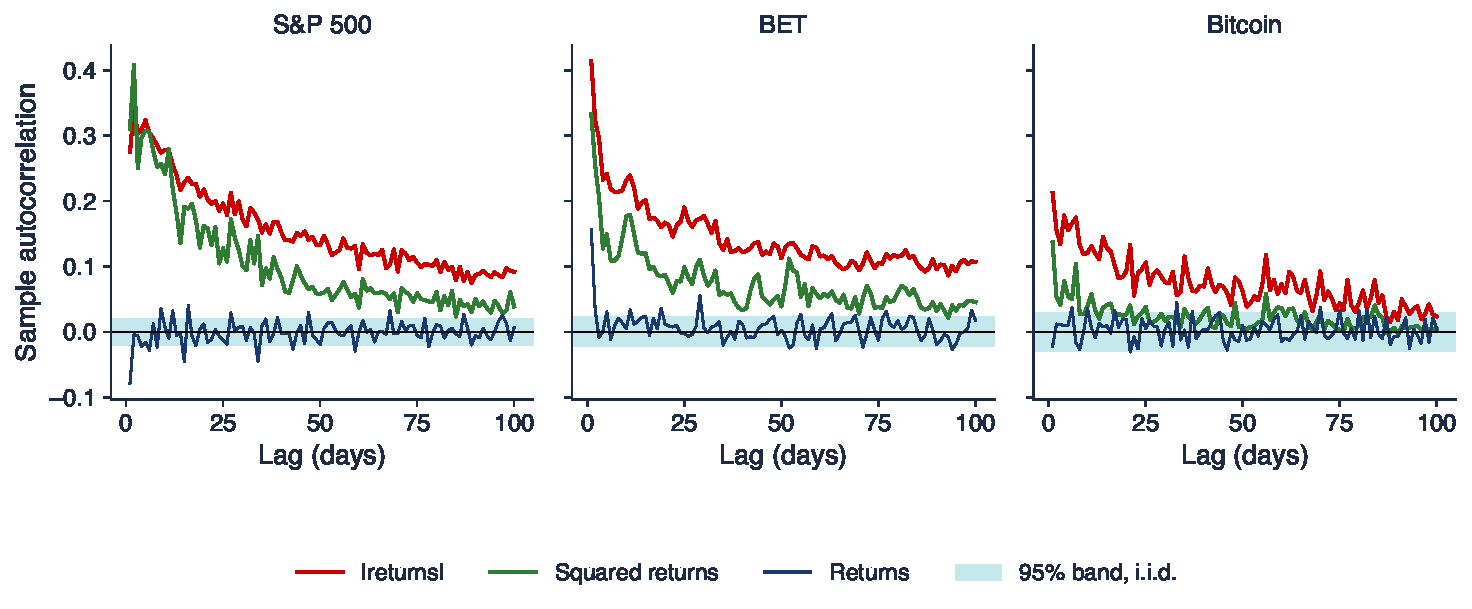
\includegraphics[width=0.97\textwidth,height=0.52\textheight,keepaspectratio]{sfm_ch8_acf_clustering.pdf}
\end{center}
\vspace{-0.25cm}
\begin{itemize}
    \item Sample ACF (autocorrelation function, \sfmchlink{https://danpele.github.io/SFM/EN/Courses/chapter7_efficient_markets_random_walk_vr.pdf}{Chapter 7}) of $r_t$, $r_t^2$ and $|r_t|$, lags 1--100, with the 95\% band $\pm 1.96/\sqrt{T}$ for i.i.d.\ data
    \item S\&P 500: all 100 autocorrelations of $r_t^2$ and of $|r_t|$ lie above the band; at lag 100, $|r_t|$ still has $0.09$
\end{itemize}
\sfmquantlet{Ch_08}{SFM_ch8_clustering}
\end{frame}

\begin{frame}{Interpretation: Clustering in Three Markets}
\itemsize{\footnotesize}
\begin{center}
\footnotesize
\begin{tabular}{lrrrrrr}
\toprule
& $\hat\rho_1(|r|)$ & $\hat\rho_{10}(|r|)$ & $\hat\rho_{100}(|r|)$ & $\hat\rho_1(r^2)$ & $\hat\rho_{10}(r^2)$ & \textbf{Lags outside, $|r|$} \\
\midrule
S\&P 500 & $0.27$ & $0.28$ & $0.09$ & $0.31$ & $0.24$ & 100/100 \\
BET & $0.41$ & $0.23$ & $0.11$ & $0.33$ & $0.18$ & 100/100 \\
Bitcoin & $0.21$ & $0.12$ & $0.02$ & $0.14$ & $0.04$ & 92/100 \\
\bottomrule
\end{tabular}
\end{center}
\begin{itemize}
    \item Slow decay: a shock to volatility is still visible after months; Chapter 11 calls this long memory
    \item \textbf{Taylor effect}: $|r_t|$ is more autocorrelated than $r_t^2$ (96\% of lags for the S\&P 500, all lags for the BET and Bitcoin) \refDGE
    \item Bitcoin: weaker clustering in $r_t^2$ (26 of 100 lags outside the band): a few huge days dominate the squares
\end{itemize}\sfmquantlet{Ch_08}{SFM_ch8_clustering}
\end{frame}

\begin{frame}{Is Clustering Real? Shuffle the Days}
\itemsize{\footnotesize}
\begin{center}
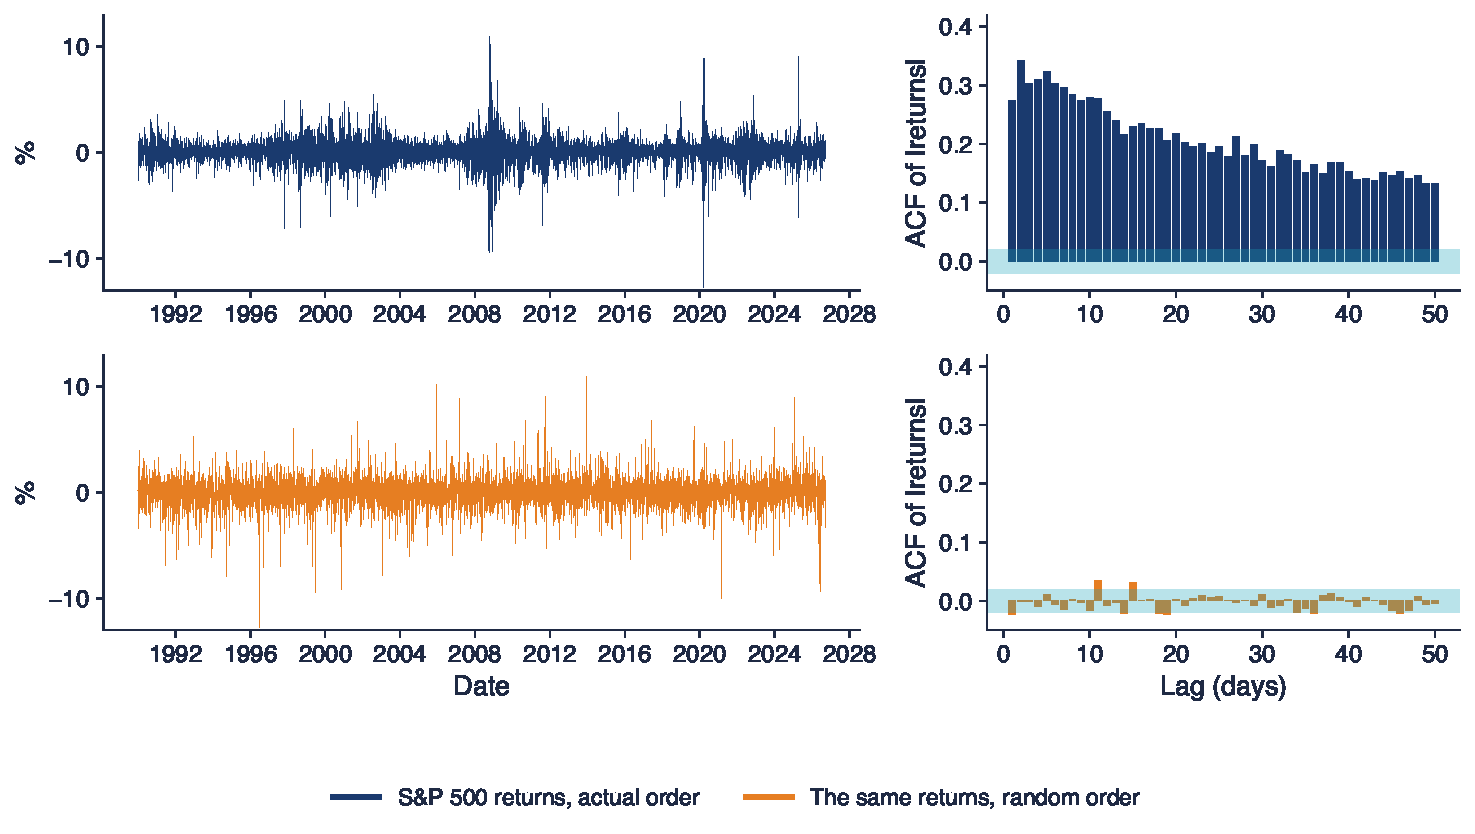
\includegraphics[width=0.97\textwidth,height=0.48\textheight,keepaspectratio]{sfm_ch8_shuffle.pdf}
\end{center}
\vspace{-0.25cm}
\begin{itemize}
    \item The same S\&P 500 returns in a random order: same distribution and same kurtosis (excess 10.9), but no clustering
    \item $\hat\rho_1(|r|)$: $0.27$ in the actual order, $-0.02$ after shuffling; Ljung--Box $Q(10)$ of $r_t^2$: 8\,015 against 6.3
    \item Clustering is a property of the \textbf{order} of the returns, not of their distribution
\end{itemize}
\sfmquantlet{Ch_08}{SFM_ch8_clustering}
\end{frame}

\begin{frame}{Testing for Clustering: Ljung--Box on Squared Returns}
\itemsize{\small}
\begin{itemize}
    \item $H_0$: no clustering, $\mathrm{Var}(r_t \mid \mathcal{F}_{t-1})$ constant, so $r_t^2$ is uncorrelated
    \begin{itemize}
        \item \textbf{McLeod--Li test} \refML: the Ljung--Box statistic \refLjung{} applied to $r_t^2$
        \item $Q(m) = T(T+2)\sum_{k=1}^m \hat\rho_k(r^2)^2/(T-k) \sim \chi^2(m)$ under $H_0$; reject if $Q(m)$ exceeds the 95\% quantile
    \end{itemize}
    \item \textbf{Worked example}: S\&P 500, $T = 9\,240$, $m = 3$
    \begin{itemize}
        \item $\hat\rho_1, \hat\rho_2, \hat\rho_3$ of $r_t^2$: $0.311$, $0.408$, $0.250$
        \item terms $T(T+2)\hat\rho_k^2/(T-k)$: 892, 1\,540, 579; $Q(3) = 3\,012 \gg \chi^2_{0.95}(3) = 7.81$: reject $H_0$
    \end{itemize}
    \item The same test on $r_t$ (\sfmchlink{https://danpele.github.io/SFM/EN/Courses/chapter7_efficient_markets_random_walk_vr.pdf}{Chapter 7}) asks a different question: is the \textbf{mean} predictable?
\end{itemize}\sfmquantlet{Ch_08}{SFM_ch8_clustering}
\end{frame}

\begin{frame}{The ARCH-LM Test (Engle, 1982)}
\itemsize{\small}
\begin{itemize}
    \item Auxiliary regression of the squared demeaned returns $e_t^2$, $e_t = r_t - \bar r$, on $q$ of their own lags \refEngle:
    \begin{itemize}
        \item $e_t^2 = c_0 + c_1 e_{t-1}^2 + \dots + c_q e_{t-q}^2 + u_t$; $H_0$: $c_1 = \dots = c_q = 0$
        \item \textbf{LM} (Lagrange multiplier) statistic: $\mathrm{LM} = n R^2 \sim \chi^2(q)$, $n$ = number of observations in the regression
    \end{itemize}
    \item S\&P 500, $q = 5$: $R^2 = 0.241$, $n = 9\,235$
    \begin{itemize}
        \item $\mathrm{LM} = 9\,235 \times 0.241 = 2\,227 \gg \chi^2_{0.95}(5) = 11.07$: strong ARCH effects
    \end{itemize}
    \item Interpretation of $R^2$: about a quarter of the day-to-day variation of $e_t^2$ is predictable from the last five days
    \item Both tests are diagnostics: they say that clustering exists, not how to model it (\sfmchlink{https://danpele.github.io/SFM/EN/Courses/chapter9_arch_garch_models.pdf}{Chapter 9})
\end{itemize}\sfmquantlet{Ch_08}{SFM_ch8_clustering}
\end{frame}

\begin{frame}{Clustering Tests in Six Series}
\itemsize{\footnotesize}
\begin{center}
\scriptsize
\begin{tabular}{lrrrrrrrr}
\toprule
& $T$ & $\hat\rho_1(r)$ & $Q(10)$, $r$ & $\hat\rho_1(r^2)$ & $Q(10)$, $r^2$ & $Q(10)$, $|r|$ & ARCH-LM(5) & \textbf{Exc.\ kurt.} \\
\midrule
S\&P 500 & 9\,240 & ${-0.079}$ & $90.8$ & $0.311$ & 8\,015 & 8\,323 & 2\,227 & $10.9$ \\
DAX & 9\,288 & ${-0.009}$ & $21.8$ & $0.155$ & 3\,747 & 5\,794 & 1\,209 & $6.0$ \\
BET & 7\,243 & ${0.156}$ & $198.3$ & $0.333$ & 2\,500 & 5\,184 & 1\,057 & $9.9$ \\
Bitcoin & 4\,384 & ${-0.022}$ & $20.2$ & $0.137$ & 213 & 1\,086 & 115 & $12.0$ \\
TLV & 3\,788 & ${0.010}$ & $29.1$ & $0.122$ & 481 & 1\,179 & 253 & $13.5$ \\
SNP & 3\,815 & ${-0.015}$ & $20.7$ & $0.195$ & 505 & 944 & 234 & $8.9$ \\
\bottomrule
\end{tabular}
\end{center}
\begin{itemize}
    \item 5\% critical values: $\chi^2_{0.95}(10) = 18.31$ for $Q(10)$, $\chi^2_{0.95}(5) = 11.07$ for ARCH-LM(5); every statistic on $r^2$ and $|r|$ rejects with p $<$ 0.001
    \item $Q(10)$ on $r$ is far smaller: mean predictability is weak (\sfmchlink{https://danpele.github.io/SFM/EN/Courses/chapter7_efficient_markets_random_walk_vr.pdf}{Chapter 7}), size predictability is strong everywhere
    \item Bitcoin and the two BVB stocks have the smallest ARCH-LM values despite heavy tails: a few extreme days dilute the regression
\end{itemize}\sfmquantlet{Ch_08}{SFM_ch8_clustering}
\end{frame}

\begin{frame}{Clustering Creates Heavy Tails}
\itemsize{\footnotesize}
\begin{center}
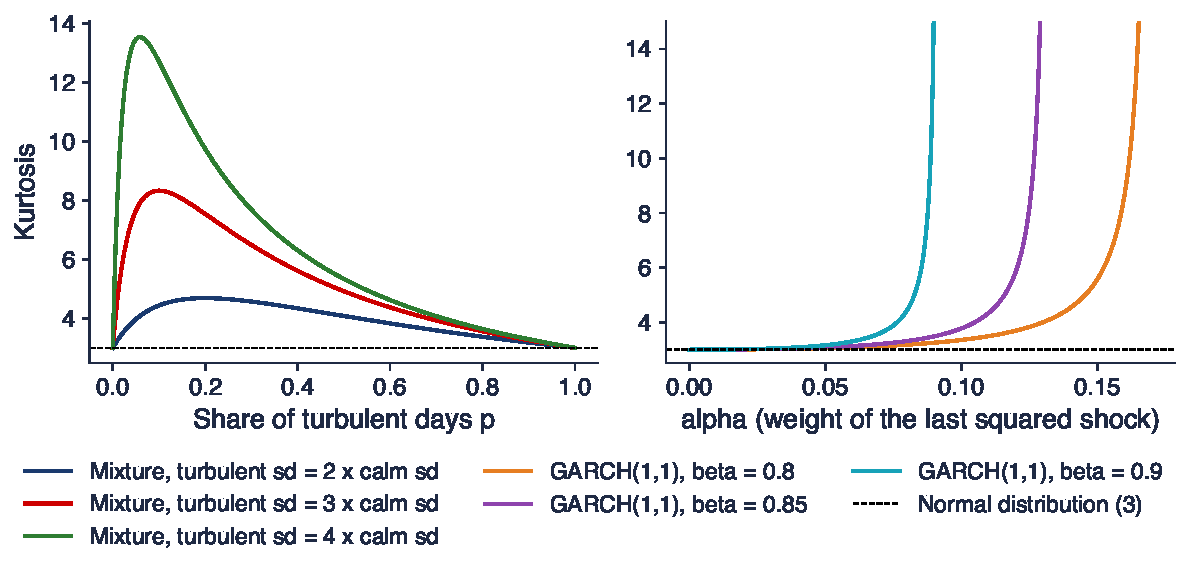
\includegraphics[width=0.97\textwidth,height=0.56\textheight,keepaspectratio]{sfm_ch8_kurtosis.pdf}
\end{center}
\vspace{-0.25cm}
\begin{itemize}
    \item Left: calm days with sd 1, turbulent days with sd 2 (share $p = 0.2$): $E[\sigma^2] = 1.6$, $E[\sigma^4] = 4.0$, kurtosis $3E[\sigma^4]/E[\sigma^2]^2 = 4.69$, though each day is Normal
    \item Right: GARCH(1,1) kurtosis $3 + 6\alpha^2/(1 - \beta^2 - 2\alpha\beta - 3\alpha^2)$, as in SFEkurgarch; $\alpha = 0.10$, $\beta = 0.85$: 3.77 (\sfmchlink{https://danpele.github.io/SFM/EN/Courses/chapter9_arch_garch_models.pdf}{Chapter 9})
\end{itemize}
\sfmquantlet{Ch_08}{SFM_ch8_kurgarch}
\end{frame}

\begin{frame}{Recap: Volatility Clustering}
\itemsize{\small}
\begin{itemize}
    \item $r_t$ almost uncorrelated, $|r_t|$ and $r_t^2$ strongly and persistently correlated: clustering
    \item Tests: Ljung--Box on $r_t^2$ (McLeod--Li) and ARCH-LM $= nR^2$; both reject in every market
    \item Clustering is about the order of returns, and it is one source of heavy tails
\end{itemize}
\end{frame}


%=============================================================================
\section{Long-Run Behaviour, the VIX and the Leverage Effect}
%=============================================================================

\begin{frame}{Volatility over Three Decades}
\itemsize{\footnotesize}
\begin{center}
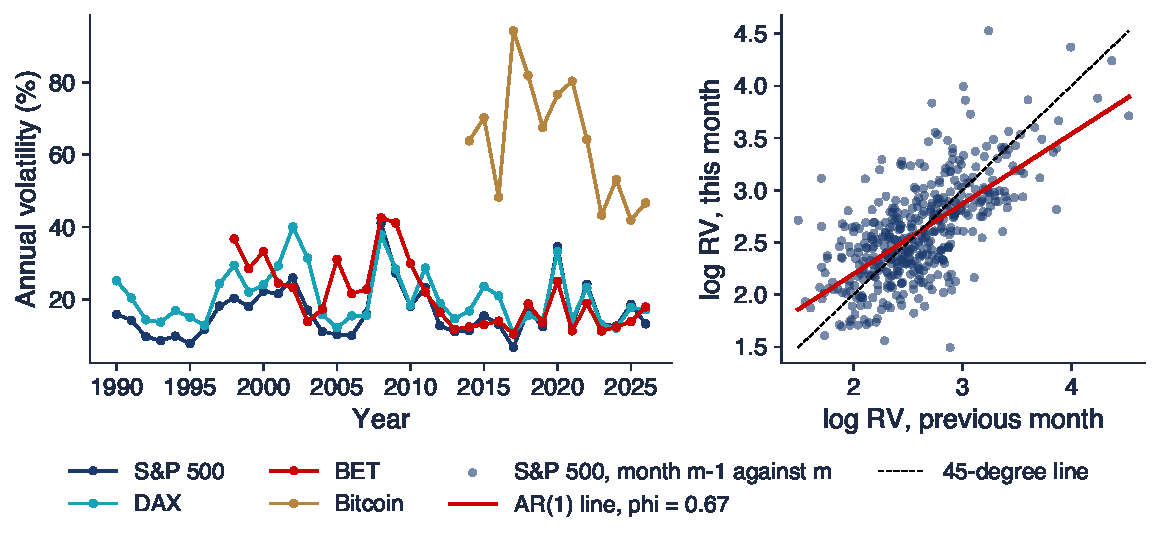
\includegraphics[width=0.97\textwidth,height=0.50\textheight,keepaspectratio]{sfm_ch8_long_term.pdf}
\end{center}
\vspace{-0.25cm}
\begin{itemize}
    \item Left: volatility of each calendar year (annualised, \%); right: log monthly realised volatility of the S\&P 500 (from daily returns) against the previous month
    \item S\&P 500: from 7\% (2017) to 41\% (2008); BET: 10\% (2017) to 43\% (2008); Bitcoin: 42\% (2025) to 94\% (2017)
\end{itemize}
\sfmquantlet{Ch_08}{SFM_ch8_long_term_vix}
\end{frame}

\begin{frame}{Interpretation: Persistence and Mean Reversion}
\itemsize{\small}
\begin{itemize}
    \item Volatility changes over time, but it does not drift away: it returns to a normal level \refSchwert
    \begin{itemize}
        \item AR(1) of log monthly realised volatility of the S\&P 500 (441 months): $\hat\phi = 0.67$ (SE 0.04)
        \item half-life of a volatility shock: $\ln 0.5/\ln\hat\phi = 1.7$ months; long-run level about 13.5\%
    \end{itemize}
    \item Monthly volatility is right-skewed (skewness 3.3), its logarithm much less (0.6) \refABDE
    \begin{itemize}
        \item mean 15.3\% above the median 12.9\%: a few crisis months pull the mean up
        \item models of volatility are therefore often written for $\ln\sigma_t$
    \end{itemize}
    \item Mean reversion is what EWMA lacks and GARCH with $\alpha + \beta < 1$ has (\sfmchlink{https://danpele.github.io/SFM/EN/Courses/chapter9_arch_garch_models.pdf}{Chapter 9})
\end{itemize}\sfmquantlet{Ch_08}{SFM_ch8_long_term_vix}
\end{frame}

\begin{frame}{The VIX: Implied Volatility}
\itemsize{\small}
\begin{columns}[T]
\begin{column}{0.58\textwidth}
\begin{itemize}
    \item Options trade on exchanges since 1973, when members of the Chicago Board of Trade founded the \textbf{CBOE} (Chicago Board Options Exchange)
    \begin{itemize}
        \item an option price depends on the volatility the market expects until expiry
        \item \textbf{implied volatility}: the volatility that, put into an option-pricing formula, gives the observed price
    \end{itemize}
    \item \textbf{VIX}, introduced in 1993 \refWhaley: the expected volatility of the S\&P 500 over the next 30 calendar days, from S\&P 500 option prices \refCboe
    \begin{itemize}
        \item quoted in annualised \%: VIX $= 20$ means about $20/\sqrt{12} \approx 5.8\%$ over a month
        \item called the ``fear index'': it jumps when stocks fall \refWhaleyB
    \end{itemize}
\end{itemize}
\end{column}
\begin{column}{0.38\textwidth}
\centering
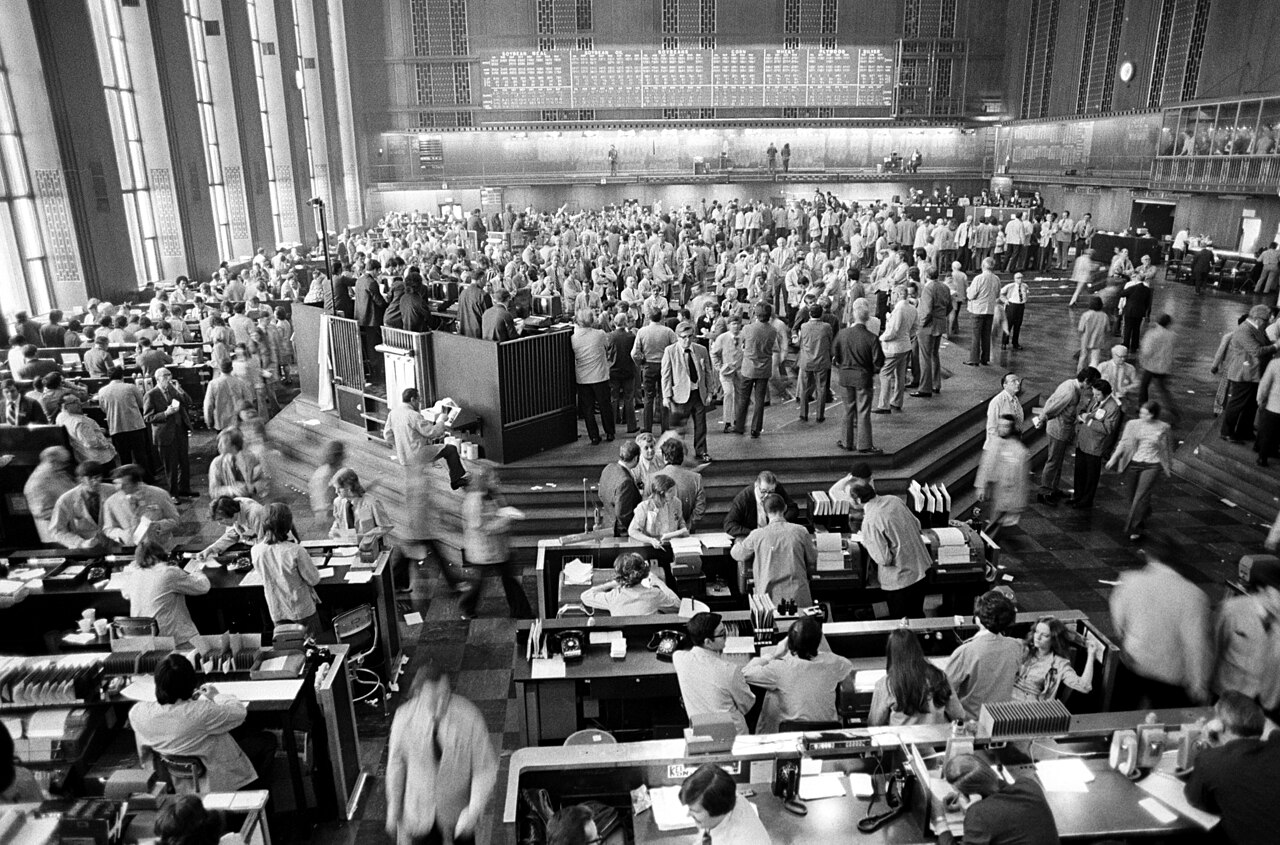
\includegraphics[height=0.34\textheight]{ch8_cbot_1973.jpg}\\[1mm]
\imgcap{Traders at the Chicago Board of Trade, 31 May 1973}
\imgcredit{https://commons.wikimedia.org/wiki/File:20120105-OC-AMW-0425_(7042322619).jpg}{Photo: U.S. Department of Agriculture (1973); public domain; Wikimedia Commons}
\end{column}
\end{columns}
\end{frame}

\begin{frame}{VIX against the Volatility That Followed}
\itemsize{\footnotesize}
\begin{center}
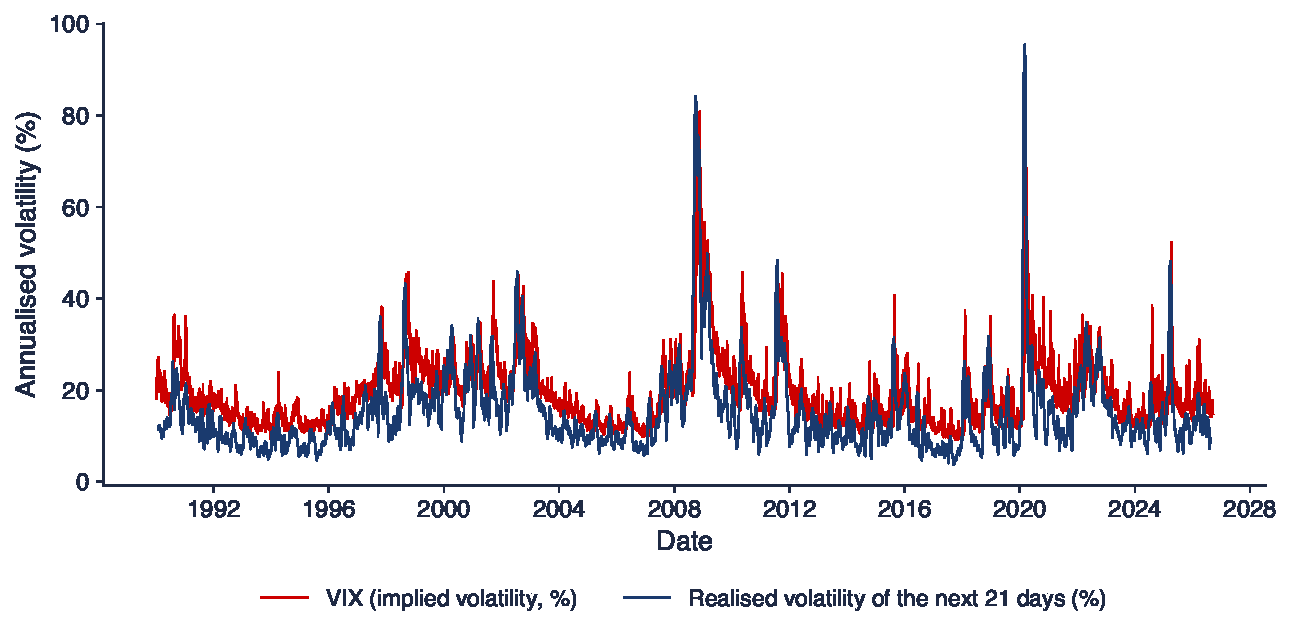
\includegraphics[width=0.97\textwidth,height=0.52\textheight,keepaspectratio]{sfm_ch8_vix.pdf}
\end{center}
\vspace{-0.25cm}
\begin{itemize}
    \item VIX and the realised volatility of the S\&P 500 over the next 21 trading days, $\sqrt{(a/21)\sum_{j=1}^{21} r_{t+j}^2}$; maximum VIX: 82.7 on 16 March 2020
    \item \textbf{Question for the room}: is the red line usually above or below the blue one?
\end{itemize}
\sfmquantlet{Ch_08}{SFM_ch8_long_term_vix}
\end{frame}

\begin{frame}{Interpretation: Implied against Realised Volatility}
\itemsize{\small}
\begin{itemize}
    \item \textbf{Answer}: above; VIX exceeded the next 21 days' realised volatility on 86\% of the 9\,199 days
    \begin{itemize}
        \item mean VIX 19.4\% against mean realised 15.3\%: a gap of 4.1 points
        \item \textbf{variance risk premium}: investors pay to be insured against volatility spikes \refCW, \refBTZ
    \end{itemize}
    \item As a forecast, VIX is informative but biased
    \begin{itemize}
        \item regression of future on implied: realised $= -1.72 + 0.88\,$VIX, $R^2 = 0.52$
        \item the past 21-day realised volatility explains less: $R^2 = 0.44$
    \end{itemize}
    \item Daily log changes of the VIX and S\&P 500 returns: correlation $-0.71$: fear rises when prices fall
\end{itemize}\sfmquantlet{Ch_08}{SFM_ch8_long_term_vix}
\end{frame}

\begin{frame}{The Leverage Effect}
\itemsize{\small}
\begin{itemize}
    \item \textbf{Leverage effect}: negative returns are followed by higher volatility than positive returns of the same size \refChristie
    \begin{itemize}
        \item leverage story: a falling share price raises the debt-to-equity ratio, so the equity becomes riskier
        \item volatility-feedback story: higher expected volatility raises the required return, so the price falls today \refFSS, \refBW
    \end{itemize}
    \item A simple measure: $\mathrm{corr}(r_t, |r_{t+j}|)$ for $j = 1, 2, \dots$
    \begin{itemize}
        \item negative: today's fall announces tomorrow's turbulence; zero under a symmetric model
    \end{itemize}
    \item \sfmchlink{https://danpele.github.io/SFM/EN/Courses/chapter2_classical_distributions_stylised_facts.pdf}{Chapter 2} met the asymmetry of the distribution; here the asymmetry is in the \textbf{dynamics} of volatility
\end{itemize}
\end{frame}

\begin{frame}{Bad News Raises Future Volatility}
\itemsize{\footnotesize}
\begin{center}
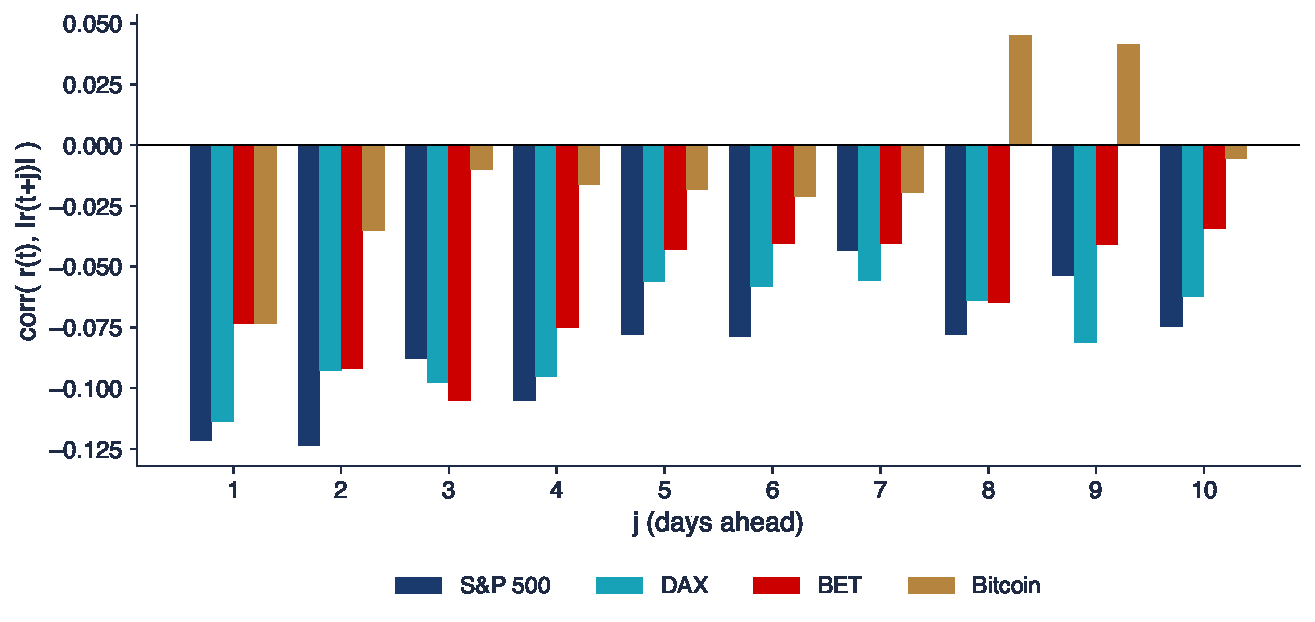
\includegraphics[width=0.97\textwidth,height=0.52\textheight,keepaspectratio]{sfm_ch8_leverage.pdf}
\end{center}
\vspace{-0.25cm}
\begin{itemize}
    \item $\mathrm{corr}(r_t, |r_{t+j}|)$, $j = 1, \dots, 10$; S\&P 500: $-0.122$ at $j = 1$; the reverse direction $\mathrm{corr}(|r_{t-1}|, r_t) = 0.025$
    \item Mean $r_{t+1}^2$ after a down day divided by that after an up day: S\&P 500 1.51, DAX 1.46, BET 1.41, Bitcoin 1.06
\end{itemize}
\sfmquantlet{Ch_08}{SFM_ch8_leverage}
\end{frame}

\begin{frame}{Nonparametric Volatility Given Yesterday's Return}
\itemsize{\footnotesize}
\begin{center}
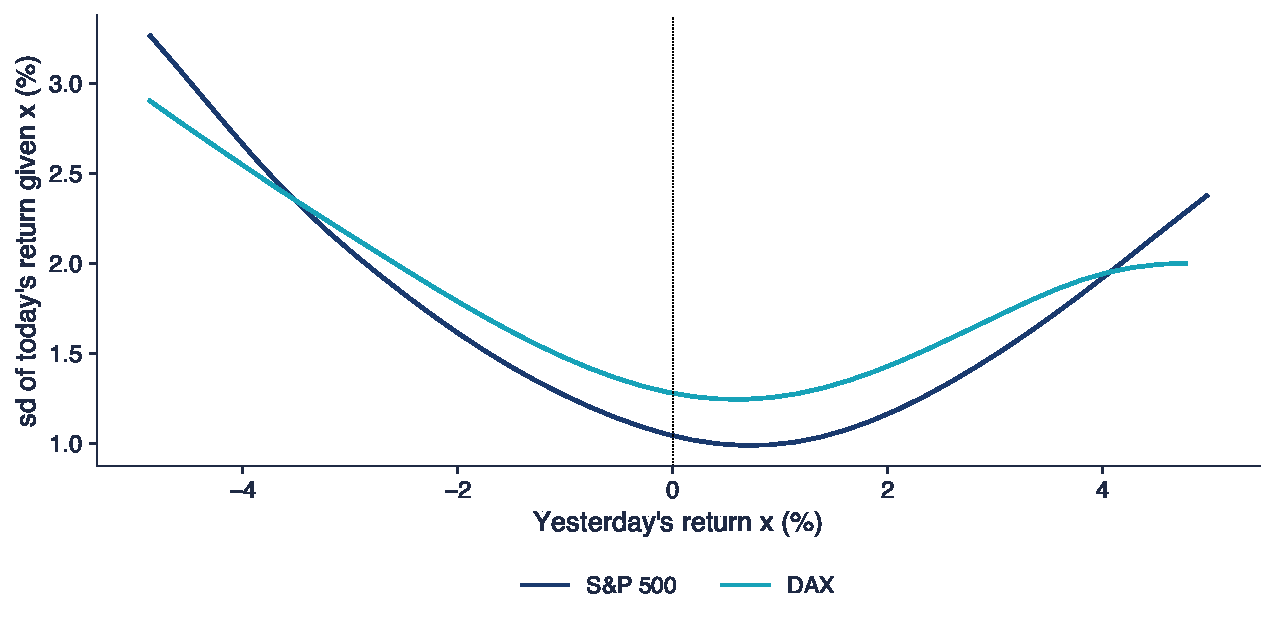
\includegraphics[width=0.97\textwidth,height=0.48\textheight,keepaspectratio]{sfm_ch8_news_impact.pdf}
\end{center}
\vspace{-0.25cm}
\begin{itemize}
    \item $\hat\sigma(x) = \sqrt{\hat m_2(x) - \hat m_1(x)^2}$, $\hat m_1$, $\hat m_2$: local linear regressions of $r_t$ and $r_t^2$ on $r_{t-1} = x$ (quartic kernel, bandwidth $0.04$ on decimal returns, as in SFEvolnonparest)
    \item S\&P 500: $\hat\sigma(-2\%) = 1.61\%$ against $\hat\sigma(+2\%) = 1.16\%$; the minimum is at $x \approx 0.7\%$, not at 0: an asymmetric news impact
\end{itemize}
\sfmquantlet{Ch_08}{SFM_ch8_leverage}
\end{frame}

\begin{frame}{Recap: Long-Run Behaviour, the VIX and the Leverage Effect}
\itemsize{\small}
\begin{itemize}
    \item Volatility is persistent but mean-reverting: half-life of about 1.7 months for the S\&P 500
    \item VIX (implied) is above realised volatility on 86\% of days: a variance risk premium
    \item Leverage effect: falls raise future volatility in equity indices; weaker and shorter-lived for Bitcoin
\end{itemize}
\end{frame}


%=============================================================================
\section{Evaluating Volatility Forecasts}
%=============================================================================

\begin{frame}{The Proxy Problem}
\itemsize{\small}
\begin{itemize}
    \item A forecast $h_t$ of $\sigma_t^2$ is made at the close of day $t-1$; the true $\sigma_t^2$ is never observed
    \begin{itemize}
        \item we compare $h_t$ with a \textbf{proxy} $\hat\sigma_t^2$: a measurable quantity with $E[\hat\sigma_t^2 \mid \mathcal{F}_{t-1}] = \sigma_t^2$
    \end{itemize}
    \item Proxies, from noisy to precise: $r_t^2$, a range estimator, realised variance
    \begin{itemize}
        \item with $r_t^2$ even a perfect forecast looks poor: \refAB{} showed that a low $R^2$ does not mean a bad model
    \end{itemize}
    \item \textbf{Mincer--Zarnowitz regression} \refMZ: $\hat\sigma_t^2 = a + b\,h_t + u_t$
    \begin{itemize}
        \item a good forecast has $a \approx 0$, $b \approx 1$; the $R^2$ measures how much of the proxy the forecast explains
    \end{itemize}
\end{itemize}
\end{frame}

\begin{frame}{Loss Functions: MSE and QLIKE}
\itemsize{\small}
\begin{itemize}
    \item Average loss over the evaluation days; lower is better \refPatton
    \begin{itemize}
        \item MSE: $L = (\hat\sigma_t^2 - h_t)^2$
        \item \textbf{QLIKE} (quasi-likelihood): $L = \hat\sigma_t^2/h_t + \ln h_t$, minus the Normal log-likelihood up to constants
    \end{itemize}
    \item Both are \textbf{robust}: with a noisy but unbiased proxy they rank forecasts as the true variance would
    \begin{itemize}
        \item losses on $\sqrt{h_t}$ or on $\ln h_t$ are not robust and can prefer the wrong forecast
    \end{itemize}
    \item \textbf{Worked example}: true variance and proxy equal to 1; two forecasts, $h = 0.5$ and $h = 2$
    \begin{itemize}
        \item MSE: $(1 - 0.5)^2 = 0.25$ against $(1 - 2)^2 = 1$: MSE punishes over-prediction more
        \item QLIKE: $1/0.5 + (-0.693) = 1.307$ against $1/2 + 0.693 = 1.193$: QLIKE punishes under-prediction more, the costly error for risk management
    \end{itemize}
\end{itemize}
\end{frame}

\begin{frame}{S\&P 500: Which Forecast Is Best?}
\itemsize{\footnotesize}
\begin{center}
\footnotesize
\begin{tabular}{lrrrrrr}
\toprule
& \textbf{21 days} & \textbf{63 days} & \textbf{252 days} & \textbf{EWMA 0.94} & \textbf{EWMA 0.97} & \textbf{VIX} \\
\midrule
MSE & 18.99 & 20.77 & 21.43 & 17.77 & 19.02 & 16.70 \\
QLIKE & 0.876 & 0.914 & 1.099 & 0.808 & 0.844 & 0.799 \\
MZ $R^2$, proxy $r^2$ & 0.14 & 0.05 & 0.01 & 0.17 & 0.11 & 0.25 \\
MZ $R^2$, range proxy & 0.24 & 0.09 & 0.02 & 0.29 & 0.19 & 0.42 \\
\bottomrule
\end{tabular}
\end{center}
\begin{itemize}
    \item Next-day variance forecasts for 4\,202 days from 2010; proxy $r_t^2$; VIX forecast: VIX$^2/a$; range proxy: $o_t^2$ plus the Garman--Klass term
    \item \textbf{DM} (Diebold--Mariano) test of equal QLIKE \refDM: EWMA 0.94 against 21 days $t = -4.50$ (p $<$\,0.001); VIX against EWMA 0.94 $t = -0.32$ (p = 0.751)
    \item EWMA beats the 21-day window; VIX and EWMA are not significantly different; the long window is worst; a precise proxy raises every $R^2$, but not the ranking
\end{itemize}\sfmquantlet{Ch_08}{SFM_ch8_forecast_evaluation}
\end{frame}

\begin{frame}{Forecasts in 2020}
\itemsize{\footnotesize}
\begin{center}
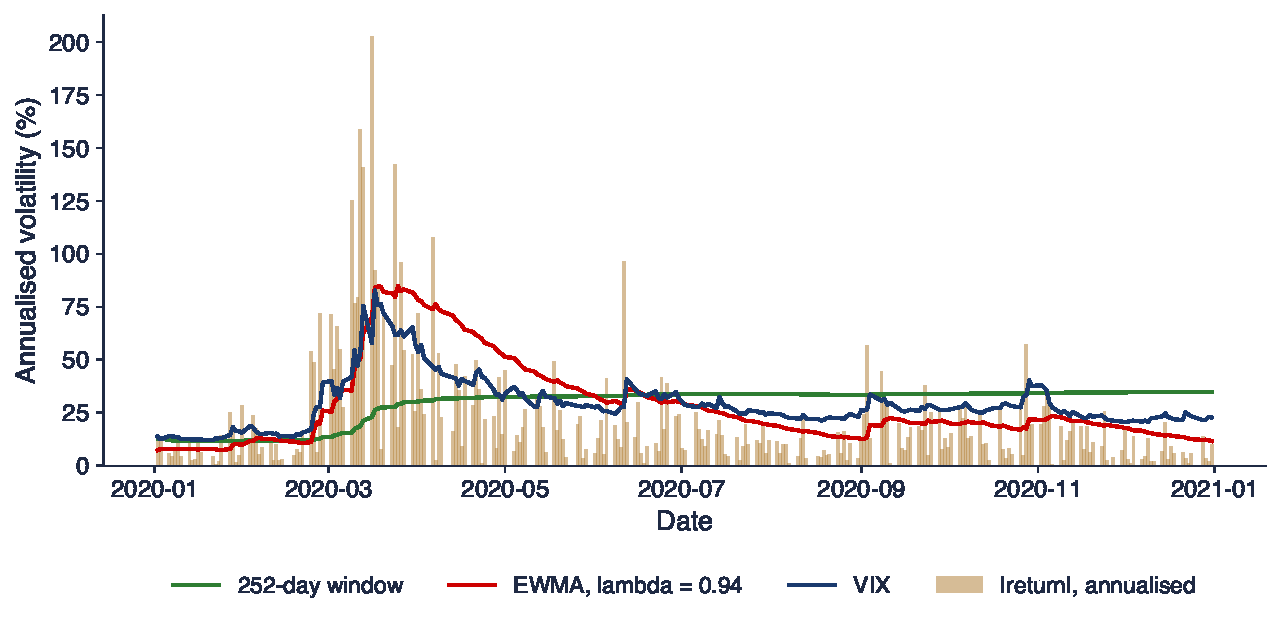
\includegraphics[width=0.97\textwidth,height=0.52\textheight,keepaspectratio]{sfm_ch8_forecast_paths.pdf}
\end{center}
\vspace{-0.25cm}
\begin{itemize}
    \item Next-day volatility forecasts of the S\&P 500 in 2020 (annualised): 252-day window, EWMA ($\lambda = 0.94$) and VIX; bars: $|r_t|$
    \item VIX started to rise one trading day before the first large fall of February 2020; EWMA rose right after it; the 252-day window moved slowly and stayed near its peak for the rest of the year
\end{itemize}
\sfmquantlet{Ch_08}{SFM_ch8_forecast_evaluation}
\end{frame}

\begin{frame}{Choosing $\lambda$ by QLIKE}
\itemsize{\footnotesize}
\begin{center}
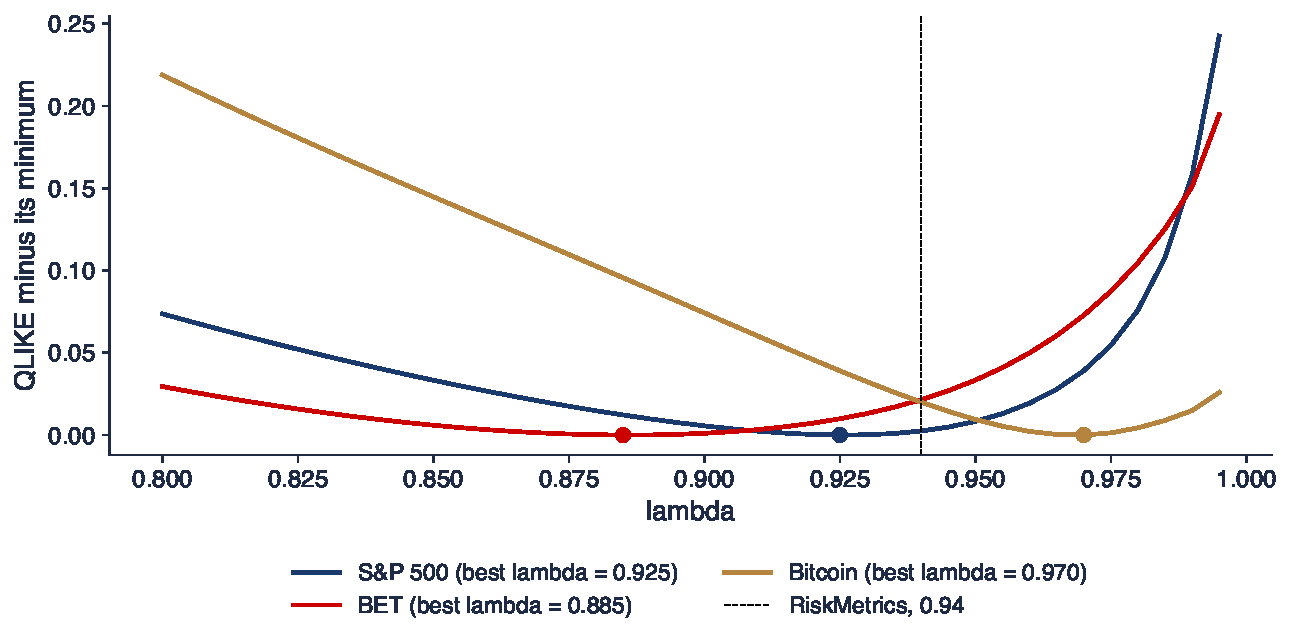
\includegraphics[width=0.97\textwidth,height=0.48\textheight,keepaspectratio]{sfm_ch8_lambda.pdf}
\end{center}
\vspace{-0.25cm}
\begin{itemize}
    \item Mean QLIKE of next-day EWMA forecasts (proxy $r_t^2$, from 2010; Bitcoin from 2016) minus its minimum, for $\lambda$ from 0.80 to 0.995
    \item Best $\lambda$: S\&P 500 0.925, BET 0.885, Bitcoin 0.970; the RiskMetrics 0.94 loses only 0.002 for the S\&P 500
    \item One $\lambda$ for all assets is a convenient compromise, not an optimum
\end{itemize}
\sfmquantlet{Ch_08}{SFM_ch8_forecast_evaluation}
\end{frame}

\begin{frame}{Recap: Evaluating Volatility Forecasts}
\itemsize{\small}
\begin{itemize}
    \item Compare forecasts with a proxy; $r_t^2$ is unbiased but noisy, so $R^2$ values are low even for good forecasts
    \item Use robust losses (MSE, QLIKE) and test the differences (Diebold--Mariano); a large comparison of volatility models: \refHL
    \item S\&P 500: EWMA and VIX are the best simple forecasts; long windows are the worst
\end{itemize}
\end{frame}


%=============================================================================
\section{AI for Scientific Discovery}
%=============================================================================

\begin{frame}{An Open Question}
\itemsize{\small}
\begin{itemize}
    \item \textbf{Do range-based estimators help on the Bucharest Stock Exchange, where many stocks trade thinly?}
    \begin{itemize}
        \item theory: ranges are 5 to 9 times more efficient; but thin trading shrinks the observed range (Section 4)
        \item days with trades but an unchanged close, since 2010: TLV 9\%, SNP 8\%, BRD 10\%, TGN 10\%
        \item Parkinson / close-to-close volatility: TLV 0.81, SNP 0.87, BRD 0.90, TGN 0.87 (S\&P 500: 0.78)
        \item QLIKE of next-day forecasts by the 21-day window, CC against YZ: TLV 2.022 against 2.039; TGN 1.750 against 1.636
    \end{itemize}
    \item Open: the answer differs by stock; is it liquidity, the opening auction, or the size of the overnight move?
    \item AI tools can speed up such a study; they do not replace checking it \refWang
\end{itemize}\sfmquantlet{Ch_08}{SFM_ch8_bvb_range}
\end{frame}

\begin{frame}{How AI Could Help}
\itemsize{\small}
\begin{itemize}
    \item \textbf{Literature}: list studies of range-based and realised volatility in emerging and thin markets, with their data and estimators
    \item \textbf{Code}: a first draft of the five estimators, rolling forecasts and QLIKE comparisons for all BET stocks
    \item \textbf{Robustness}: liquidity groups by volume, other windows, the 2016--2020 and 2021--2026 halves
    \item Example prompt
    \begin{itemize}
        \item \aiprompt{Write a Python function that computes the Parkinson, Garman-Klass, Rogers-Satchell and Yang-Zhang variance on rolling 21-day windows from daily open, high, low and close prices, and compares their next-day forecasts with QLIKE against squared close-to-close returns.}
    \end{itemize}
\end{itemize}
\end{frame}

\begin{frame}{What to Check}
\itemsize{\small}
\begin{itemize}
    \item The constants: $4\ln 2$ in Parkinson, $2\ln 2 - 1$ in Garman--Klass, $k$ in Yang--Zhang; a draft with $\ln 2$ or $k = 0.34$ is wrong
    \item Stock prices: open, high and low must be adjusted for dividends and splits with the same factor as the close
    \item Annualisation with the actual frequency: 365 for crypto, about 250 for BVB stocks
    \item No look-ahead: the forecast for day $t$ uses only data up to day $t-1$
    \item References: every cited paper must exist; check the DOI
\end{itemize}
\end{frame}

\begin{frame}{Project Idea}
\itemsize{\small}
\begin{itemize}
    \item \textbf{Question}: which daily volatility estimator should a Romanian risk manager use?
    \begin{itemize}
        \item data: BVB stocks since 2010 (TLV, SNP, BRD, TGN, and others with OHLC data), S\&P 500 and DAX as benchmarks (EODHD)
    \end{itemize}
    \item Steps
    \begin{itemize}
        \item the five estimators on 21-day windows; EWMA versions of each; next-day forecasts
        \item QLIKE and MSE with the proxy $r_t^2$; Diebold--Mariano tests; results by liquidity group
        \item relate the gain of YZ over CC to the share of zero-volume days and to the overnight share
    \end{itemize}
    \item Deliverables: one table, one chart, and a paragraph on what the data can and cannot show
    \item Declare any AI use, and list the errors of the AI that you corrected
\end{itemize}
\end{frame}


%=============================================================================
\section{Summary}
%=============================================================================

\begin{frame}{Key Takeaways}
\itemsize{\small}
\begin{itemize}
    \item Volatility is the standard deviation of returns; it is latent and changes over time; annualise with the actual frequency
    \item Historical windows trade speed against noise; EWMA ($\lambda = 0.94$) reacts fast and avoids ghosts
    \item Range estimators use the daily path: far more efficient, but biased by overnight jumps and thin trading; Yang--Zhang adds the night
    \item Clustering: $|r_t|$ and $r_t^2$ are autocorrelated; detect it with Ljung--Box on $r_t^2$ and ARCH-LM
    \item Volatility mean-reverts; VIX usually exceeds realised volatility; falls raise future volatility
    \item Compare forecasts with robust losses (QLIKE) and a proxy; test the differences
\end{itemize}
\end{frame}

\begin{frame}{Key Formulas}
\itemsize{\small}
{\renewcommand{\arraystretch}{1.4}\begin{center}
\scriptsize
\begin{tabular}{ll}
\toprule
\textbf{Quantity} & \textbf{Formula} \\
\midrule
Annualised volatility & $\sigma_{\text{year}} = \sigma_{\text{day}}\sqrt{a}$ \\
EWMA & $\sigma_t^2 = \lambda\sigma_{t-1}^2 + (1-\lambda)r_{t-1}^2$, \quad half-life $\ln 0.5/\ln\lambda$ \\
Parkinson & $(u_t - d_t)^2/(4\ln 2)$ \\
Garman--Klass & $0.5(u_t - d_t)^2 - (2\ln 2 - 1)c_t^2$ \\
Rogers--Satchell & $u_t(u_t - c_t) + d_t(d_t - c_t)$ \\
Yang--Zhang & $\hat\sigma_O^2 + k\hat\sigma_C^2 + (1-k)\hat\sigma_{RS}^2$, \quad $k = 0.34/(1.34 + (n+1)/(n-1))$ \\
Realised variance & $\mathrm{RV}_t = \sum_i r_{t,i}^2$ \\
McLeod--Li & $Q(m) = T(T+2)\sum_{k=1}^m \hat\rho_k(r^2)^2/(T-k) \sim \chi^2(m)$ \\
ARCH-LM & $\mathrm{LM} = nR^2 \sim \chi^2(q)$ \\
MSE, QLIKE & $(\hat\sigma_t^2 - h_t)^2$, \quad $\hat\sigma_t^2/h_t + \ln h_t$ \\
\bottomrule
\end{tabular}
\end{center}
}
\end{frame}

\begin{frame}{Check Yourself}
\itemsize{\small}
\begin{itemize}
    \item \textbf{Question}: a stock has $H = 102$, $L = 98$ on one day; what is the Parkinson daily volatility?
    \begin{itemize}
        \item \textbf{Answer}: $\ln(102/98) = 4.00\%$; $\sqrt{4.00^2/2.77} = 2.40\%$
    \end{itemize}
    \item \textbf{Question}: Ljung--Box on returns does not reject, on squared returns it rejects strongly; what do you conclude?
    \begin{itemize}
        \item \textbf{Answer}: the mean is unpredictable, the variance is predictable: volatility clustering without autocorrelation
    \end{itemize}
    \item \textbf{Question}: why can EWMA with $\lambda = 0.94$ not forecast a return of volatility to its normal level?
    \begin{itemize}
        \item \textbf{Answer}: $\alpha + \beta = 1$ and $\omega = 0$: its forecasts are flat at every horizon
    \end{itemize}
    \item Next: \sfmchlink{https://danpele.github.io/SFM/EN/Courses/chapter9_arch_garch_models.pdf}{Chapter 9}, ARCH and GARCH models
\end{itemize}
\end{frame}


%=============================================================================
\section{References}
%=============================================================================

\begin{frame}{References (1/3)}
\itemsize{\tiny}
\begin{itemize}
    \item Alizadeh, S., Brandt, M.W., Diebold, F.X. (2002). \href{https://doi.org/10.1111/1540-6261.00454}{Range-based estimation of stochastic volatility models}. \textit{Journal of Finance}, 57(3), 1047--1091.
    \item Andersen, T.G., Bollerslev, T. (1998). \href{https://doi.org/10.2307/2527343}{Answering the skeptics: yes, standard volatility models do provide accurate forecasts}. \textit{International Economic Review}, 39(4), 885--905.
    \item Andersen, T.G., Bollerslev, T., Diebold, F.X., Ebens, H. (2001). \href{https://doi.org/10.1016/S0304-405X(01)00055-1}{The distribution of realized stock return volatility}. \textit{Journal of Financial Economics}, 61(1), 43--76.
    \item Andersen, T.G., Bollerslev, T., Diebold, F.X., Labys, P. (2003). \href{https://doi.org/10.1111/1468-0262.00418}{Modeling and forecasting realized volatility}. \textit{Econometrica}, 71(2), 579--625.
    \item Barndorff-Nielsen, O.E., Shephard, N. (2002). \href{https://doi.org/10.1111/1467-9868.00336}{Econometric analysis of realized volatility and its use in estimating stochastic volatility models}. \textit{Journal of the Royal Statistical Society, Series B}, 64(2), 253--280.
    \item Bekaert, G., Wu, G. (2000). \href{https://doi.org/10.1093/rfs/13.1.1}{Asymmetric volatility and risk in equity markets}. \textit{Review of Financial Studies}, 13(1), 1--42.
    \item Bollerslev, T. (1986). \href{https://doi.org/10.1016/0304-4076(86)90063-1}{Generalized autoregressive conditional heteroskedasticity}. \textit{Journal of Econometrics}, 31(3), 307--327.
    \item Bollerslev, T., Tauchen, G., Zhou, H. (2009). \href{https://doi.org/10.1093/rfs/hhp008}{Expected stock returns and variance risk premia}. \textit{Review of Financial Studies}, 22(11), 4463--4492.
    \item Borak, S., Härdle, W.K., López-Cabrera, B. (2013). \href{https://doi.org/10.1007/978-3-642-33929-5}{\textit{Statistics of Financial Markets: Exercises and Solutions}}, 2nd ed. Springer.
    \item Carr, P., Wu, L. (2009). \href{https://doi.org/10.1093/rfs/hhn038}{Variance risk premiums}. \textit{Review of Financial Studies}, 22(3), 1311--1341.
    \item Cboe Global Markets (2026). \href{https://www.cboe.com/tradable_products/vix/}{Cboe Volatility Index (VIX)}. Product page and methodology.
    \item Christie, A.A. (1982). \href{https://doi.org/10.1016/0304-405X(82)90018-6}{The stochastic behavior of common stock variances: value, leverage and interest rate effects}. \textit{Journal of Financial Economics}, 10(4), 407--432.
    \item Cont, R. (2001). \href{https://doi.org/10.1080/713665670}{Empirical properties of asset returns: stylized facts and statistical issues}. \textit{Quantitative Finance}, 1(2), 223--236.
    \item Corsi, F. (2009). \href{https://doi.org/10.1093/jjfinec/nbp001}{A simple approximate long-memory model of realized volatility}. \textit{Journal of Financial Econometrics}, 7(2), 174--196.
    \item Diebold, F.X., Mariano, R.S. (1995). \href{https://doi.org/10.1080/07350015.1995.10524599}{Comparing predictive accuracy}. \textit{Journal of Business \& Economic Statistics}, 13(3), 253--263.
    \item Ding, Z., Granger, C.W.J., Engle, R.F. (1993). \href{https://doi.org/10.1016/0927-5398(93)90006-D}{A long memory property of stock market returns and a new model}. \textit{Journal of Empirical Finance}, 1(1), 83--106.
\end{itemize}
\end{frame}

\begin{frame}{References (2/3)}
\itemsize{\tiny}
\begin{itemize}
    \item Engle, R.F. (1982). \href{https://doi.org/10.2307/1912773}{Autoregressive conditional heteroscedasticity with estimates of the variance of United Kingdom inflation}. \textit{Econometrica}, 50(4), 987--1007.
    \item Engle, R.F. (2004). \href{https://doi.org/10.1257/0002828041464597}{Risk and volatility: econometric models and financial practice}. \textit{American Economic Review}, 94(3), 405--420.
    \item Franke, J., Härdle, W.K., Hafner, C.M. (2019). \href{https://doi.org/10.1007/978-3-030-13751-9}{\textit{Statistics of Financial Markets: An Introduction}}, 5th ed. Springer.
    \item French, K.R., Schwert, G.W., Stambaugh, R.F. (1987). \href{https://doi.org/10.1016/0304-405X(87)90026-2}{Expected stock returns and volatility}. \textit{Journal of Financial Economics}, 19(1), 3--29.
    \item Garman, M.B., Klass, M.J. (1980). \href{https://doi.org/10.1086/296072}{On the estimation of security price volatilities from historical data}. \textit{Journal of Business}, 53(1), 67--78.
    \item Hansen, P.R., Lunde, A. (2005). \href{https://doi.org/10.1002/jae.800}{A forecast comparison of volatility models: does anything beat a GARCH(1,1)?} \textit{Journal of Applied Econometrics}, 20(7), 873--889.
    \item J.P. Morgan/Reuters (1996). \href{https://www.msci.com/documents/10199/5915b101-4206-4ba0-aee2-3449d5c7e95a}{\textit{RiskMetrics -- Technical Document}}, 4th ed. New York: Morgan Guaranty Trust Company.
    \item Liu, L.Y., Patton, A.J., Sheppard, K. (2015). \href{https://doi.org/10.1016/j.jeconom.2015.02.008}{Does anything beat 5-minute RV? A comparison of realized measures across multiple asset classes}. \textit{Journal of Econometrics}, 187(1), 293--311.
    \item Ljung, G.M., Box, G.E.P. (1978). \href{https://doi.org/10.1093/biomet/65.2.297}{On a measure of lack of fit in time series models}. \textit{Biometrika}, 65(2), 297--303.
    \item Mandelbrot, B. (1963). \href{https://doi.org/10.1086/294632}{The variation of certain speculative prices}. \textit{Journal of Business}, 36(4), 394--419.
    \item McLeod, A.I., Li, W.K. (1983). \href{https://doi.org/10.1111/j.1467-9892.1983.tb00373.x}{Diagnostic checking ARMA time series models using squared-residual autocorrelations}. \textit{Journal of Time Series Analysis}, 4(4), 269--273.
    \item Mincer, J.A., Zarnowitz, V. (1969). \href{https://www.nber.org/books-and-chapters/economic-forecasts-and-expectations-analysis-forecasting-behavior-and-performance/evaluation-economic-forecasts}{The evaluation of economic forecasts}. In J.A. Mincer (ed.), \textit{Economic Forecasts and Expectations}, 3--46. NBER.
    \item Molnár, P. (2012). \href{https://doi.org/10.1016/j.irfa.2011.06.012}{Properties of range-based volatility estimators}. \textit{International Review of Financial Analysis}, 23, 20--29.
    \item Nobel Prize Outreach (2003). \href{https://www.nobelprize.org/prizes/economic-sciences/2003/summary/}{The Sveriges Riksbank Prize in Economic Sciences in Memory of Alfred Nobel 2003: Robert F. Engle III and Clive W.J. Granger}. nobelprize.org.
    \item Parkinson, M. (1980). \href{https://doi.org/10.1086/296071}{The extreme value method for estimating the variance of the rate of return}. \textit{Journal of Business}, 53(1), 61--65.
    \item Patton, A.J. (2011). \href{https://doi.org/10.1016/j.jeconom.2010.03.034}{Volatility forecast comparison using imperfect volatility proxies}. \textit{Journal of Econometrics}, 160(1), 246--256.
\end{itemize}
\end{frame}

\begin{frame}{References (3/3)}
\itemsize{\tiny}
\begin{itemize}
    \item Pele, D.T., Lazar, E., Dufour, A. (2017). \href{https://doi.org/10.3390/e19050226}{Information entropy and measures of market risk}. \textit{Entropy}, 19(5), 226.
    \item Pele, D.T., Mazurencu-Marinescu-Pele, M. (2019). \href{https://doi.org/10.3390/e21020102}{Using high-frequency entropy to forecast Bitcoin's daily Value at Risk}. \textit{Entropy}, 21(2), 102.
    \item Poon, S.-H., Granger, C.W.J. (2003). \href{https://doi.org/10.1257/002205103765762743}{Forecasting volatility in financial markets: a review}. \textit{Journal of Economic Literature}, 41(2), 478--539.
    \item Rogers, L.C.G., Satchell, S.E. (1991). \href{https://doi.org/10.1214/aoap/1177005835}{Estimating variance from high, low and closing prices}. \textit{Annals of Applied Probability}, 1(4), 504--512.
    \item Schwert, G.W. (1989). \href{https://doi.org/10.1111/j.1540-6261.1989.tb02647.x}{Why does stock market volatility change over time?} \textit{Journal of Finance}, 44(5), 1115--1153.
    \item Tsay, R.S. (2010). \href{https://doi.org/10.1002/9780470644560}{\textit{Analysis of Financial Time Series}}, 3rd ed. Wiley.
    \item Wang, H., Fu, T., Du, Y., Gao, W., et al. (2023). \href{https://doi.org/10.1038/s41586-023-06221-2}{Scientific discovery in the age of artificial intelligence}. \textit{Nature}, 620, 47--60.
    \item Whaley, R.E. (1993). \href{https://doi.org/10.3905/jod.1993.407868}{Derivatives on market volatility}. \textit{Journal of Derivatives}, 1(1), 71--84.
    \item Whaley, R.E. (2009). \href{https://doi.org/10.3905/JPM.2009.35.3.098}{Understanding the VIX}. \textit{Journal of Portfolio Management}, 35(3), 98--105.
    \item Yang, D., Zhang, Q. (2000). \href{https://doi.org/10.1086/209650}{Drift-independent volatility estimation based on high, low, open, and close prices}. \textit{Journal of Business}, 73(3), 477--492.
\end{itemize}
\end{frame}

\end{document}
